%%%%%%%%%%%%%%%%%%%%%%%%%%%%%%%%%%%%%%%%%%%%%%%%%%%%%%%%%%%%%%%%%%%%%%
% Lớp 11 | Đường thẳng, mặt phẳng. Quan hệ song song trong | Đường thẳng và mặt phẳng song song
% Dạng 1H4?3-4: Tìm giao điểm của đường thẳng và mặt phẳng
% Số câu: 31  (sinh tự động bởi tach_cau.py; từ nay thầy sửa trực tiếp file này)
%%%%%%%%%%%%%%%%%%%%%%%%%%%%%%%%%%%%%%%%%%%%%%%%%%%%%%%%%%%%%%%%%%%%%%

%%%%%%%%%%%%%%%% TRẮC NGHIỆM 4 PHƯƠNG ÁN %%%%%%%%%%%%%%%%

% nguồn: Ok_TracNghiemLop11_Lan1
\begin{ex}%[1H4N3-4]%[ma:8fc7109a]
	\immini{Cho tứ diện $ABCD$. Gọi $G$ là trọng tâm của tam giác $ACD$. Giao điểm của đường thẳng $CD$ và mặt phẳng $(ABG)$ là 
	\choice 
		{\True điểm $M$ (với  $M$ là trung điểm của $CD$)}
		{điểm  $C$}
		{điểm $D$} 
		{điểm  $G$}}
		 {
		\begin{tikzpicture}[scale=.7]
				\def\a{4} 
				\path  (0:0) coordinate (B)
					++(0:\a)  coordinate (D)
					 ++(-140:.6*\a) coordinate (C)
					($(B)+(70:\a)$)  coordinate (A)
					 ($(C)!.5!(D)$) coordinate (M)
					($(A)!2/3!(M)$)  coordinate (G);
				 \draw[dashed] (G)--(B)--(D);
				 \draw (B)--(A)--(D)
					 (A)--(C)
					(B)--(C)--(D) 
					 (A)--(G);
				\foreach \x/\g in {A/90,B/180,C/-45,D/0,G/0} 
				\fill[black]  (\x) circle (1pt)
					($(\g:3mm)+(\x)$) node {$\x$}; 
			\end{tikzpicture}
		} 
	 \loigiai{
	\immini{Trong  mặt phẳng $(ACD)$, gọi $M$ là giao điểm của $AG$ và $CD$.\\
		Do $G$ là trọng tâm của tam giác $ACD$ nên $M$ là  trung điểm của $CD$.\\
		Ta có $\heva{&M\in CD\\&M\in AG;\; AG\subset(ABG)} \Rightarrow (ABG)\cap CD=\left\{M\right\}$.} 
		{\begin{tikzpicture}[scale=.7]
		 \def\a{4}
		\path (0:0) coordinate (B) 
			++(0:\a) coordinate (D) 
			++(-140:.6*\a) coordinate (C) 
			($(B)+(70:\a)$)  coordinate (A)
			($(C)!.5!(D)$) coordinate  (M)
			($(A)!2/3!(M)$) coordinate  (G);
		\draw[dashed]  (G)--(B)--(D);
		 \draw (B)--(A)--(D)
			 (A)--(C)
			(B)--(C)--(D) 
			 (A)--(M);
		\foreach \x/\g in {A/90,B/180,C/-45,D/0,G/0,M/-45} 
		\fill[black] (\x) circle (1pt) 
			 ($(\g:3mm)+(\x)$) node {$\x$};
	\end{tikzpicture}
		} 
	 }
\end{ex}

% nguồn: Ok_Toan11_TracNghiem_Lan2
\begin{ex}%[1H4H3-4]%[ma:68f4ce79]
	Cho hình chóp $S.ABCD$ có đáy là hình bình hành tâm $O$.  $M$ là một điểm bất kì thuộc cạnh $SC$, $H$ là giao điểm của $AM$ và mặt phẳng $\left(SBD\right)$. Trong các khẳng định sau khẳng định nào đúng?
	 \choice
		{$ H$ là giao điểm của $ AM$  và $ SD$}
		{$ H$  là giao điểm của $ AM$ và $ SB$}
		{$ H$ là  giao điểm của $ AM$ và $ BD$}
		{\True  $ H$ là giao điểm của $ AM$ và $ SO$}
	\loigiai{ 
		\begin{center}
			\begin{tikzpicture}[declare function={gocx=80; goc=-150; a=4.5; b=a/2; h=5;}]
					 \path (0,0) coordinate (A)--+(gocx:h) coordinate (S)
						(a,0)  coordinate (B)
						(goc:b)  coordinate (D)
						+(a,0) coordinate  (C)
						 ($(S)!.4!(C)$) coordinate (M)
						(intersection of A--C and B--D)  coordinate (O)
						(intersection of S--O and A--M)  coordinate (H);
					 \draw[dashed] (S)--(A)
						 (D)--(A)--(B)--(D)
						(A)--(M) 
						(A)--(C) 
						 (S)--(O);
					\draw  (S)--(D)--(C)--(S)--(B)--(C)--cycle;
					\foreach \x/\goc in  {S/90,A/150,B/0,C/-60,D/-180,O/-90,H/0,M/0}
					\draw[fill=black] (\x) node[shift={(\goc:7pt)},font=\scriptsize]{$\x$}  circle (1pt);
				\end{tikzpicture}
		\end{center}
		Gọi $  O=AC\cap BD$. Ta có $\left(SAC\right)\cap\left(SBD\right)=SO$.\\
		Trong mặt phẳng $\left(SAC\right)$, kẻ $ AM\cap  SO=\left\{ H\right\}$\\
		Ta có $\left\{\begin{array}{l}
		 H\in AM\\
		 H\in SO\subset\left(SBD\right)
	\end{array}\right.\Rightarrow H=AM\cap\left(SBD\right)$.}
\end{ex}

% nguồn: Ok_Toan11_TracNghiem_Lan2
\begin{ex}%[1H4H3-4]%[ma:e8f892cb]
	Cho hình chóp $S\cdot ABCD$  có đáy $ABCD$ là hình bình hành tâm $O$, $M$ là trung điểm đoạn $SB$, $G$ là trọng tâm tam giác $SAD$. Gọi $J$ là giao điểm của $AD$ với $(OMG)$ khi đó $\dfrac{JD}{AD}$ bằng
	 \choice
		 {$\dfrac{2}{5}$}
		 {$\dfrac{1}{4}$}
		{$\dfrac{2}{3}$} 
		{\True  $\dfrac{1}{3}$}
	 \loigiai{
		\begin{center}
			\begin{tikzpicture}[scale=1,font=\footnotesize,line join=round,line cap=round,>=stealth]
					 \path
						(0,0) coordinate  (A)
						(5,0) coordinate  (D)
						(-1.2,-1.5)  coordinate (B)
						(1,3.5) coordinate  (S)
						 ($(B)+(D)-(A)$) coordinate (C)
						 ($(B)!.5!(D)$) coordinate (O)
						 ($(S)!.5!(B)$) coordinate (M)
						($(S)!.5!(D)$)  coordinate (E)
						($(A)!2/3!(E)$) coordinate (G) 
						($(A)!2/3!(D)$) coordinate  (J)
						($(A)!2/3!(S)$)  coordinate (K);
					 \draw (S)--(B)--(C)--(D)--(S)--(C);
					\draw [dashed] (C)--(A)--(D)--(B)--(A)--(S) 
						(M)--(G)--(O)--(M) 
						(A)--(E) 
						(J) --(K); 
					\foreach  \d/\g in {A/135,B/-135,C/-45,D/45,S/90,M/135,O/-90,E/45,J/45,G/90}
					\fill  (\d) circle (1pt) + (\g:.3) node{$\d$};
					\fill[pattern=north east lines] (M)--(O)--(G)--cycle; 
				\end{tikzpicture}
		\end{center}
		Ta có $MO$ là đường  trung bình của tam giác $SBD$ suy ra $MO\parallel SD$.\\
		Ta có $\heva{&MO\parallel SD\\&G\in(OMG)\cap(SAD)}\Rightarrow(OMG)\cap(SAD)=Gx\parallel SD\parallel  MO\Rightarrow Gx\cap AD=\{J\}$.\\
		Ta  có $J\in Gx\subset(OMG)\Rightarrow J=AD\cap(OMG)$.\\
		Gọi $E$ là  trung điểm $SD$ với $G$ là trọng tâm ta có $\dfrac{AG}{AE}=\dfrac{2}{3}$.\\
		Do $GJ\parallel MO\parallel SD$ áp dụng định  lý Talet trong tam giác $AED$ ta có $\dfrac{GE}{AE}=\dfrac{JD}{AD}=\dfrac{1}{3}$.
	} 
\end{ex}

% nguồn: Ok_Toan11_TracNghiem_Lan2
\begin{ex}%[1H4H3-4]%[ma:e666f142]
	Cho tứ diện $ABCD$, có độ dài các cạnh đôii một khác nhau. Gọi $M$, $N$, $P$ lần lượt là trung điểm các cạnh $AB$, $AC$, $CD$. Mặt phẳng $(MNP)$  cắt $BD$ tại điểm $Q$. Phát biểu nào sau đây \textbf{sai}?
	\choice 
		{\True  $MN=MQ$}
		{$MQ=NP$} 
		 {$PQ\parallel (ABC)$}
		 {$MQ\parallel (ACD)$}
	\loigiai{ 
		\begin{center}
			\begin{tikzpicture}[scale=1,font=\footnotesize,line join=round,line cap=round,>=stealth]
					\path 
						(0,0) coordinate  (B)
						(5,0)  coordinate (C)
						(1.2,-1.5) coordinate (D) 
						(1,3.5)  coordinate (A)
						($(D)!.5!(C)$)  coordinate (P)
						 ($(B)!.5!(A)$) coordinate (M)
						($(B)!.5!(D)$) coordinate (Q) 
						($(A)!.5!(C)$)  coordinate (N);
					 \draw (A)--(B)--(D)--(C)--(A)--(D)
						 (Q)--(M)
						 (N)--(P);
					\draw [dashed] (C)--(B) 
						 (P)--(M)--(N)
						 (Q)--(P);
					\foreach  \d/\g in {A/90,B/135,C/45,D/-90,M/135,N/45,P/-45,Q/-135}
					\fill (\d) circle (1pt) +  (\g:.3) node{$\d$};
				\end{tikzpicture}
		\end{center}
		Ta có $MN=\dfrac{1}{2}BC$; $MQ=\dfrac{1}{2}AD\Rightarrow MQ\neq MN$ do $BC\neq  AD$.
	} 
\end{ex}

% nguồn: Ok_Toan11_TracNghiem_Lan2
\begin{ex}%[1H4H3-4]%[ma:f21292c0]
	Cho hình chóp $S.ABCD$ có đáy là hình bình hành. Gọi  $M$ là trung điểm của $SA$. Giao điểm của đường thẳng $SB$ và mặt phẳng ($CMD$) là
	\begin{center}
		\begin{tikzpicture}[scale=1,font=\footnotesize,line join=round,line cap=round,>=stealth]
				\path 
					(0,0) coordinate (A) 
					(5,0)  coordinate (B)
					(-2,-1.5)  coordinate (D)
					(1,3.5) coordinate  (S)
					($(B)+(D)-(A)$)  coordinate (C)
					($(S)!.5!(A)$) coordinate  (M);
				\draw (S)--(D)--(C)--(B)--(S)--(C); 
				\draw [dashed] (S)--(A)--(B) 
					(A)--(D)  --(M)--(C);
				\foreach \d/\g in  {A/135,D/-135,C/-45,B/45,S/90,M/0}
				\fill  (\d) circle (1pt) + (\g:.3) node{$\d$};
			\end{tikzpicture}
	\end{center}
	\choice 
		{Không có giao  điểm}
		{Giao điểm của đường thẳng  $SB$ và $MC$}
		{Giao điểm của  đường thẳng $SB$ và $MD$}
		{\True Trung  điểm của đoạn thẳng $SB$}
	\loigiai{ 
		\begin{center}
			\begin{tikzpicture}[scale=1,font=\footnotesize,line join=round,line cap=round,>=stealth]
					\path 
						(0,0)  coordinate (A)
						 (5,0) coordinate (B)
						 (-2,-1.5) coordinate (D)
						(.5,3.5)  coordinate (S)
						($(B)+(D)-(A)$) coordinate  (C)
						($(S)!.5!(A)$)  coordinate (M)
						($(S)!.5!(B)$) coordinate (N); 
					 \draw (S)--(D)--(C)--(B)--(S)--(C)--(N);
					 \draw [dashed] (S)--(A)--(B)
						(A)--(D)  --(M)--(C)
						(M)--(N); 
					 \foreach \d/\g in {A/135,D/-135,C/-45,B/45,S/90,M/165,N/45}
					\fill (\d) circle (1pt) +  (\g:.3) node{$\d$};
				\end{tikzpicture}
		\end{center}
		Ta có $\heva{&AB\parallel CD\\&M\in(CMD)\cap(SAB)\\&CD\subset(CMD)\\&AB\subset(SAB)}$, suy  ra $(CMD)\cap(SAB)=MN\parallel AB\parallel CD$ với $N\in SB$.\\
		Khi đó $N$ là giao  điểm của đường thẳng $SB$ và mặt phẳng $(CMD)$.\\
		Xét tam giác $\triangle SAB$ có $M$ là trung điểm $SA$ và $MN\parallel AB\Rightarrow N$ là trung điểm $SB$. 
	} 
\end{ex}

% nguồn: Ok_Toan11_TracNghiem_Lan2
\begin{ex}%[1H4H3-4]%[ma:ee2593ab]
	Cho lăng trụ tam giác $ABC.A' B'  C'$. Gọi $M$, $N$ lần lượt là trung điểm của $BB'$, $CC'$. Đường thẳng qua đi qua trọng tâm $I$ của tam giác $ABC$ cắt $A'B$ và $MN$ lần lượt tại $P$, $Q$. Khi đó tỉ số $\dfrac{IP}{IQ}$ bằng
	 \choice
		{$\dfrac{3}{5}$} 
		{$\dfrac{5}{2}$} 
		{\True  $\dfrac{2}{5}$}
		 {$\dfrac{5}{3}$}
	 \loigiai{
		\begin{center}
			\begin{tikzpicture}[line join = round,line cap = round,>=stealth,font=\footnotesize,scale=.8,declare function={ab=3; ac=5.5; cao=6; gocA=-50;}]
					 \path
						(0,0)  coordinate (A')
						 (gocA:ab) coordinate (B')
						 (ac,0) coordinate (C')
						($(A')+(90:cao)$) coordinate (A) 
						($(A)+(ac,0)$)  coordinate (C)
						($(A)+(gocA:ab)$) coordinate (B) 
						($(B)!0.5!(B')$) coordinate (M) 
						($(C)!0.5!(C')$)  coordinate (N)
						($(A)!2/3!(C)$)  coordinate (K)
						($(A)!2/3!(B)$)  coordinate (H)
						($(A)!0.5!(C)$) coordinate (ac) 
						 (intersection of B--ac and H--K) coordinate (I)
						($(A')!0.5!(C')$)  coordinate (a'c')
						($(B')!2/3!(a'c')$) coordinate  (Q)
						($(A')!0.5!(B)$) coordinate  (D)
						(intersection of  A'--B and H--M) coordinate (P);
					\draw (A')--(B')--(C') 
						 (A)--(B)--(C)--cycle (A')--(A)
						 (B')--(B)
						 (C')--(C)
						(A')--(B) 
						 (M)--(H)--(K)
						 (B)--(ac)
						(M)--(N) 
						 (M)--(D);
					 \draw[dashed] (A')--(C')
						 (I)--(Q)
						 (K)--(N)
						 (M)--(Q);
					\foreach \x/\gm in {A'/180,B'/-90,C'/0,A/90,C/0,B/-30,I/180,K/90,H/180,D/180,M/-140,N/0,Q/-90,P/180} \fill  (\x) circle (1pt)
						 ($(\x)+(\gm:3.5mm)$) node{$\x$};
				\end{tikzpicture}
		\end{center}
		Qua $I$ kẻ  đường thẳng song song với $BC$ cắt $AC$, $AB$ tại $H$, $K$.\\
		Suy ra $KH\parallel MN$ do đó $M$, $N$, $K$, $H$, $I$ đồng  phẳng.\\
		Gọi $P=A'B\cap MH$,  $Q=IP\cap MN$.\\
		Kẻ $MD\parallel A' B'\left(D\in A' B\right)$ ta được $\dfrac{HP}{PM}=\dfrac{HB}{DM}=\dfrac{\dfrac{1}{3} \cdot AB}{\dfrac{1}{2}  \cdot A' B'}=\dfrac{2}{3}$.\\
		Do đó  $\dfrac{IP}{PQ}=\dfrac{HP}{PM}=\dfrac{2}{3}$ nên $\dfrac{IP}{PQ}=\dfrac{2}{5}$.
	} 
\end{ex}

% nguồn: Ok_Toan11_TracNghiem_Lan2
\begin{ex}%[1H4H3-4]%[ma:d602a238]
	Cho hình chóp $S.ABCD$ có đáy $ABCD$ là  hình bình hành. Gọi $M$, $N$ lần lượt là trung điểm $AD$ và $BC$. Giao tuyến của hai mặt phẳng $(SMN)$ và $(SAC)$ là
	 \choice
		{\True $SO$ với $O$ là tâm hình  bình hành $ABCD$}
		{$SD$} 
		 {$SG$ với $G$ là trung điểm $AB$}
		{$SF$ với $F$  là trung điểm $CD$}
	\loigiai{ 
		\begin{center}
			\begin{tikzpicture}[scale=.7,font=\footnotesize,line join=round,line cap=round,>=stealth]
					 \path
						(0,0) coordinate  (A)
						(5,0) coordinate (B) 
						(-2.5,-1.5) coordinate  (D)
						(.5,3.5) coordinate  (S)
						 ($(B)+(D)-(A)$) coordinate (C)
						($(A)!.5!(D)$) coordinate (M) 
						($(B)!.5!(C)$)  coordinate (N)
						 ($(B)!.5!(D)$) coordinate (O);
					 \draw (S)--(D)--(C)--(B)--(S)--(C)
						(S)--(N); 
					\draw  [dashed] (S)--(A)--(B)
						 (A)--(D)
						(S)--(M)--(N) 
						 (A)--(C);
					\foreach  \d/\g in {A/135,D/-135,C/-45,B/45,S/90,M/135,N/-45,O/-90}
					\fill (\d) circle (1pt) + (\g:.3)  node{$\d$};
				\end{tikzpicture}
		\end{center}
		Gọi $O$ là giao điểm  $AC$ và $MN$ ta có $\heva{&S\in(SAC)\cap(SMN)\\&O\in(SAC)\cap(SMN)}\Rightarrow SO=(SAC)\cap(SMN)$.\\
		Vì $MN\parallel AB$ và $N$ là trung điểm $BC$ nên  $O$ là trung điểm $AC\Rightarrow O$ là tâm hình bình hành $ABCD$.
	 }
\end{ex}

% nguồn: Ok_Toan11_TracNghiem_Lan2
\begin{ex}%[1H4H3-4]%[ma:db6e4453]
	Cho hình hộp $ABCD.A'B'C'D'$. Gọi $M$ là trung điểm của $AB$, mặt phẳng $\left(MA'C'\right)$ cắt cạnh $BC$ tại $N$. Tính tỉ số  $k=\dfrac{MN}{A'C'}$.
	 \choice
		{\True $k=\dfrac{1}{2}$} 
		{$k=\dfrac{1}{3}$} 
		 {$k=\dfrac{2}{3}$}
		 {$k=1$}
	 \loigiai{
		\begin{center}
			\begin{tikzpicture}[scale=0.8,font=\footnotesize,line join=round,line cap=round,>=stealth]
					\coordinate  (B) at (0,0);
					\coordinate (A) at  (-2,-2);
					 \coordinate (C) at (6,0);
					 \coordinate (D) at ($(A)+(C)-(B)$);
					\foreach \i in {A,B,C,D}{\coordinate (\i') at ($(\i)-(0,5)$);} 
					\draw  (A)--(B)--(C)--(D)--cycle;
					\draw  (A)--(A')
						(C)--(C') 
						(D)--(D') 
						 (A')--(D')--(C');
					\draw[dashed,thin] (B)--(B')--(A') 
						(B')--(C'); 
					\coordinate (M)  at ($(A)!0.5!(B)$);
					\coordinate (N)  at ($(B)!0.5!(C)$);
					\draw (M)--(N); 
					\draw[dashed,thin]  (M)--(A')--(C')--(N);
					\foreach  \i/\g in {A'/170,B'/170,C'/-90,D'/-90,A/90,B/90,C/-20,D/10,M/90,N/0}{\draw[fill=blue](\i) circle (1pt)
						($(\i)+(\g:5mm)$)  node[scale=1]{$\i$};}
				\end{tikzpicture}
		\end{center}
		Ba mặt phẳng phân biệt $\left(ABCD\right),\left(ACC'A'\right),\left(MA'C'\right)$ đôi một cắt nhau  theo ba giao tuyến $AC$, $A'C'$ và $MN$. Theo tính chất hình hộp ta có $AC \parallel A'C'$ nên $MN \parallel AC \parallel A'C'$.\\
		Lại có $M$ là trung điểm của $AB$ nên $MN$ là đường trung bình trong tam giác  $ABC$.\\
		Vì vậy $MN=\dfrac{1}{2} AC=\dfrac{1}{2}  A'C'\Rightarrow k=\dfrac{MN}{A'C'}=\dfrac{1}{2}$.
	 }
\end{ex}

% nguồn: Ok_Toan11_TracNghiem_Lan2
\begin{ex}%[1H4H3-4]%[1H4H3-4]%[1H4H3-4]%[1H4H3-4]%[1H4H3-4]%[ma:e429121c]
	Cho hình chóp $S. ABCD$ có đáy $ABCD$ là hình thang với $AB\parallel CD$ và $AB=2CD$. Gọi $G$ là trọng tâm của tam giác  $SBC, H$ là giao điểm của $DG$ và $(SAC)$. Tỉ số $\dfrac{GH}{GD}$ bằng
	\choice 
		{$\dfrac{1}{2}$} 
		{$\dfrac{3}{5}$} 
		 {\True $\dfrac{2}{5}$}
		 {$\dfrac{2}{3}$}
	\loigiai{ 
		\begin{center}
			\begin{tikzpicture}[line join = round,line cap = round,>=stealth,font=\footnotesize,scale=1,declare function={ad=2; ab=4.5; cd=ab/2; gs=80; sa=4; gocA=-50;}]
					\path 
						(0,0) coordinate (A) 
						(ab,0) coordinate (B) 
						(gocA:ad)  coordinate (D)
						 ($(D)+(cd,0)$) coordinate (C)
						 (gs:sa) coordinate (S)
						($(C)!0.5!(B)$) coordinate  (M)
						 ($(S)!2/3!(M)$) coordinate (G)
						(intersection of A--C and B--D) coordinate (N) 
						(intersection of  S--N and G--D) coordinate (H)
						 ($(S)!2/3!(N)$) coordinate (K)
						 ($(B)-(A)+(D)$) coordinate (E);
					\draw (S)--(A)--(D)--(C)--(B)--(S)--(C) 
						(S)--(D) 
						 (S)--(M)--(E)
						 (C)--(E)--(B);
					 \draw[dashed] (B)--(A)
						 (A)--(C)
						 (B)--(D)
						(S)--(N) 
						(K)--(G)--(D)--(M); 
					\foreach \x/\gm in {A/180,B/0,C/-90,D/-90,S/90,E/-90,M/-90,G/0,K/180,H/180,N/-90} \fill (\x) circle  (1pt)
						 ($(\x)+(\gm:3.5mm)$) node{$\x$};
				\end{tikzpicture}
		\end{center}
		Gọi $M$ là trung điểm của $BC, N$ là giao điểm của $AC$  và $MD$.\\
		Khi đó, $(SMD)  \cap(SAC)=SN$.\\
		Vì $DG\subset(SMD)$  và $DG\cap(SAC)=H$ nên $H\in SN$.\\
		Gọi $E$ là điểm đối xứng với $D$  qua $C$ thì tứ giác $ABED$ là hình bình hành.\\
		Suy ra $EM\parallel AC$. Do  đó, $N$ là trung điểm của $MD$.\\
		Dựng đường thẳng đi qua $G$ song song với $MN$ và cắt $SN$  tại $K$.\\
		Khi đó, $\dfrac{SG}{SM}=\dfrac{KG}{NM}$ và $\dfrac{HD}{HG}=\dfrac{DN}{KG}$.\\ 
		Suy  ra $\dfrac{SG}{SM}\cdot\dfrac{NM}{ND}\cdot\dfrac{HD}{HG}=\dfrac{KG}{NM}\cdot\dfrac{NM}{ND}\cdot\dfrac{ND}{KG}=1$.\\
		Mặt khác $\dfrac{SG}{SM}=\dfrac{1}{3}$ và $\dfrac{NM}{ND}=1$ nên $\dfrac{2}{3}\cdot 1\cdot \dfrac{HD}{HG}=1\Leftrightarrow\dfrac{HD}{HG}=\dfrac{2}{3}$.\\ 
		 Vậy $\dfrac{GH}{GD}=\dfrac{2}{5}$.
	 }
\end{ex}

% nguồn: Ok_TracNghiemLop11_Lan1
\begin{ex}%[1H4H3-4]%[ma:67950cf8]
	Cho hình chóp $ S.ABCD$ có đáy $ ABCD$ là hình bình hành. Gọi $ d$ là giao tuyến của hai mặt phẳng $\left(SAD\right)$ và $\left(SBC\right)$. Khẳng định nào sau  đây đúng?
	 \choice
		{$ d$ qua $ S$ và song song với $  BD$}
		{\True  $ d$ qua $ S$ và song song với $ BC$}
		{$ d$ qua  $ S$ và song song với $ DC$}
		{$ d$ qua $ S$ và song song với $  AB$}
	 \loigiai{
		Xét 2 mặt  phẳng $\left(SAD\right)$ và $\left(SBC\right)$.
		\begin{center}
			\begin{tikzpicture}[line join = round,line cap = round,font=\footnotesize,>=stealth,scale=1]
					\coordinate  (A) at (0,0);
					\coordinate  (C) at (5,0);
					\coordinate (B) at (2,2); 
					\coordinate (D) at  ($(B)+(C)-(A)$);
					\coordinate (S) at (3,5); 
					\coordinate (K) at  ($(C)+(S)-(A)$);
					\coordinate  (M) at ($(S)!-1!(K)$);
					\draw (K)--(S)--(A)--(C)--(D)--(S)--(C) 
						 (M)--(S);
					\draw[dashed] (A)--(B)--(D) 
						 (S)--(B);
					\foreach  \i/\g in {A/-90,B/180,C/-90,D/0,S/90}{\draw[fill](\i) circle (1pt)
						 ($(\i)+(\g:3mm)$) node[scale=1]{$\i$};}
				\end{tikzpicture}
		\end{center}
		Ta  có: $\heva{& S\in\left(SAD\right)\cap\left(SBC\right)\\
		 &AD\subset\left(SAD\right)\\
		&BC\subset\left(SBC\right)\\ 
		&AD \parallel BC 
		}$ 
	Nên giao tuyến hai mặt phẳng $\left(SAD\right)$ và $\left(SBC\right)$ là đường thẳng $ d$ qua $ S$ và song song  với $ BC$.}
\end{ex}

% nguồn: Ok_Toan11_TracNghiem_Lan2
\begin{ex}%[1H4V3-4]%[ma:7f2e8a13]
	\immini{Cho hình chóp $S.ABCD$ có đáy là  hình bình hành. Gọi $M$ là trung điểm của $SA$. Giao điểm của đường thẳng $SB$ và mặt phẳng $(CMD)$ là
	 \choice
		{Không  có giao điểm}
		{Giao điểm của  đường thẳng $SB$ và $MC$}
		{Giao điểm của đường thẳng $SB$ và  $MD$}
		{\True Trung điểm của đoạn thẳng $SB$}}{\begin{tikzpicture}[declare function={gocx=80; goc=-150; a=3; b=a/2; h=3;}]
		\path (0,0) coordinate  (A)--+(gocx:h) coordinate (S)
			(a,0) coordinate (B) 
			 (goc:b) coordinate (D)
			+(a,0)  coordinate (C)
			 ($(S)!0.5!(A)$) coordinate (M);
		\fill[gray!20]  (D)--(M)--(C)--cycle;
		\draw[dashed]  (S)--(A)
			 (D)--(A)--(B)
			(D)--(M)--(C); 
		\draw  (S)--(D)--(C)--(S)--(B)--(C)--cycle;
		\foreach  \x/\goc in {S/90,A/150,B/0,C/-60,D/-180,M/180}
		\draw[fill=black] (\x) node[shift={(\goc:7pt)},font=\scriptsize]{$\x$} circle (1pt); 
	\end{tikzpicture}
		 }
	 \loigiai{
	\immini{Ta  có
		$\heva{&AB\parallel  CD\\&M\in(CMD)\cap(SAB)\\&CD\subset(CMD), AB\subset(SAB).}$\\
		Khi đó giao tuyến của hai mặt phẳng $(CMD)$ và $(SAB)$  là đường thẳng $MN\parallel AB\parallel CD$ với $N\in SB$.\\
		Suy ra $N$ là giao điểm của đường thẳng $SB$ và mặt phẳng  $(CMD)$.\\
		Xét tam giác $\triangle SAB$ có $M$  là trung điểm $SA$ và $MN\parallel AB$.\\
		Do đó $N$ là trung điểm $SB$.}{\begin{tikzpicture}[declare function={gocx=80; goc=-150; a=3; b=a/2; h=3;}]
		\path (0,0) coordinate (A)--+(gocx:h) coordinate  (S)
			(a,0)  coordinate (B)
			(goc:b) coordinate (D) 
			+(a,0) coordinate  (C)
			($(S)!0.5!(A)$) coordinate (M) 
			($(S)!0.5!(B)$) coordinate (N); 
		\fill[gray!20]  (D)--(M)--(N)--(C)--cycle;
		 \draw[dashed] (S)--(A)
			 (D)--(A)--(B)
			 (D)--(M)--(N)--(C)
			 (M)--(C);
		 \draw (S)--(D)--(C)--(S)--(B)--(C)--cycle;
		\foreach \x/\goc in {S/90,A/150,B/0,C/-60,D/-180,M/180,N/0} 
		\draw[fill=black] (\x) node[shift={(\goc:7pt)},font=\scriptsize]{$\x$} circle (1pt); 
	\end{tikzpicture}
		 }
	 }
\end{ex}


%%%%%%%%%%%%%%%% ĐÚNG/SAI %%%%%%%%%%%%%%%%

% nguồn: Ok_dungsai_lop11_Lan1
\begin{ex}%[1H4N3-4]%[ma:351b75f2]
 Cho hình chóp $S.ABCD$ có  $AB$ và $CD$ không song song. Gọi $M$ là điểm thuộc miền trong của tam giác $SCD$.
 \choiceTF 
  {Giao điểm $N$  của đường thẳng $CD$ và mặt phẳng $\left(SBM\right)$ là giao điểm của đường thẳng $CD$ và đường thẳng $SB$}
  {Gọi $O=AC\cap BN$, giao điểm $I$ của đường thẳng $BM$ và mặt phẳng $\left(SAC\right)$ là giao điểm của đường thẳng  $BM$ và đường thẳng $SC$}
  {\True Giao điểm $P$ của đường thẳng $SC$ và mặt phẳng $\left(ABM\right)$ là giao điểm của đường thẳng $SC$ và đường thẳng $AI$} 
  {Thiết diện của hình chóp $S.ABCD$ cắt bởi  mặt phẳng $\left(ABM\right)$ là tứ giác $ABPM$}
 \loigiai{ 
  \begin{center}
   \begin{tikzpicture}[>=stealth,line join=round,line cap = round,scale=1,font=\footnotesize]
     \def\ad{6} 
      \def\ab{3}
      \def\h{4}
     \def\gocA{-60} 
     \path 
       (0,0) coordinate (A)
      (\gocA:\ab) coordinate (B) 
      ($(B)+(3,0.5)$) coordinate  (C)
       (\ad,0) coordinate (D)
      (2.5,\h) coordinate (S) 
       ($(C)!2/3!(D)$) coordinate (N)
      ($(S)!2/5!(N)$) coordinate  (M)
       (intersection of B--N and A--C) coordinate (O)
      (intersection of B--M and S--O) coordinate (I) 
      (intersection of A--I and  S--C) coordinate (P)
      (intersection of P--M and  S--D) coordinate (K);
      \fill[blue!10] (A)--(B)--(P)--(K)--cycle;
      \foreach \p/\q in {S/90,A/180,B/-90,C/-90,D/0,N/-90,M/0,K/45,I/-135,O/-90,P/0}
      \fill[black] (\p) circle (1.0pt) node[shift={(\q:3.5mm)}]{$\p$};
      \draw (S)--(D)--(C)--(S)--(A)--(B)--(C)
      (K)--(P)--(B)--(S)--(N); 
      \draw[dashed] (A)--(D)
      (A)--(P) 
       (A)--(K)
      (B)--(N) 
       (A)--(C)
      (S)--(O); 
    \end{tikzpicture}
  \end{center}
  \begin{itemchoice}
   \itemch \textbf{Sai}. Trong mặt phẳng $\left(SCD\right)$  có $SM$ cắt $CD$ tại điểm $N$ suy ra $N=CD\cap (SBM)$.
    \itemch \textbf{Sai}. Trong mặt phẳng $\left(ABCD\right)$, ta có $O=AC\cap BN$ và trong mặt phẳng $\left(SBN\right)$ có $BM$ cắt $SO$ tại điểm $I$ suy ra $I=BM\cap (SAC)$.
   \itemch \textbf{Đúng}.  Trong mặt phẳng $\left(SAC\right)$ có $SC$ cắt $AI$ tại điểm $P$ suy ra $P=SC\cap (ABM)$.
   \itemch \textbf{Sai}. Trong mặt  phẳng $\left(SCD\right)$, gọi $K=PM\cap SD$ suy ra tứ giác $ABPK$ là thiết diện cần tìm.
  \end{itemchoice}
  }
\end{ex}

% nguồn: Ok_dungsai_lop11_Lan1
\begin{ex}%[1H4H3-4]%[ma:976dbe8e]
 Cho hình chóp $S.ABCD$ có đáy $ABCD$ là hình thang đáy lớn $AB=2CD$. Gọi $O$ là giao điểm của $AC$ và $BD$,  $M$ là trung điểm $SA$.
 \choiceTF 
  {Tỉ  số $\dfrac{OA}{OC}$ bằng $\dfrac{1}{2}$}
  {\True  Nếu $N$ là giao điểm của $SB$ và $\left(MCD\right)$ thì $N$ là trung điểm $SB$}
  {\True Nếu $F$ là  giao điểm của $\left(OMN\right)$ và $AD$ thì $AF=2FD$}
  {Nếu $E$ là giao điểm của $\left(OMN\right)$ và $BC$ thì tứ giác $MNEF$ là hình thang có đáy lớn  $EF=\dfrac{5}{4}MN$}
 \loigiai{ 
  \begin{center}
   \begin{tikzpicture}[scale=1,font=\footnotesize,line join=round,line cap=round,>=stealth]
     \def\ad{3} 
      \def\ab{6}
     \def\h{4} 
      \def\gocA{-70}
     \path 
      (0,0)  coordinate (A)
      (\ab,0)  coordinate (B)
       (\gocA:\ad) coordinate (D)
      ($(D)+(3,0)$)  coordinate (C)
      (2,\h)  coordinate (S)
       (intersection of A--C and B--D) coordinate (O)
      ($(A)!2/3!(D)$)  coordinate (F)
      ($(B)!2/3!(C)$) coordinate (E) 
      ($(S)!0.5!(A)$) coordinate  (M)
      ($(S)!0.5!(B)$) coordinate (N); 
      \draw (S)--(A)--(D)--(C)--(B)--(S)--(D)--(C)--cycle (M)--(D)--(C)--(N)
      (M)--(F) 
       (N)--(E);
     \draw[dashed] (A)--(C) 
      (B)--(D) 
      (F)--(E) 
      (M)--(N)--(O)--cycle (A)--(B); 
      \foreach \p/\q in {S/90,A/180,B/0,C/-90,D/-90,E/0,F/180,M/180,N/0,O/-90}
     \fill[black] (\p) node[shift={(\q:3mm)}]{$\p$} circle (1.0pt); 
    \end{tikzpicture}
  \end{center}
  \begin{itemchoice}
   \itemch \textbf{Sai}.Ta có $AB$ song song $CD$ nên áp dụng định lí Thalès ta  có $\dfrac{OA}{OC}=\dfrac{AB}{CD}=2$.
   \itemch  \textbf{Đúng}.Ta có $N=SB\cap\left(MCD\right)$ nên $N\in\left(MCD\right)\cap\left(SAB\right)$.\\
    Mặt khác ta lại có $M\in\left(MCD\right)\cap\left(SAB\right)$ nên $MN=\left(MCD\right)\cap\left(SAB\right)$.\\
   Mà $AB$ song song $CD$ nên $MN$ song song $AB$. 
   Kết hợp $M$ là trung điểm $SA$ ta nhận được $N$ cũng là trung điểm  $SB$ do tính chất đường trung bình.
   \itemch \textbf{Đúng}. Với $F=\left(OMN\right)\cap  CD$ thì ta có $F\in\left(OMN\right)\cap\left(ABCD\right)$\\
   Mà $O\in\left(OMN\right)\cap\left(ABCD\right)$ nên  $FO=\left(OMN\right)\cap\left(ABCD\right)$.\\
   Ta lại có  $MN$ song song $AB$ nên $FO$ song song $AB$.\\
   Áp dụng định lí Thalès ta có  $\dfrac{AF}{FD}=\dfrac{AO}{OC}=2$.
   Vậy $AF=2FD$. 
   \itemch \textbf{Sai}. Chứng minh tương tự ở ý c) ta cũng được $OE$ song song $AB$ nên $O, E, F$ thẳng hàng và $EF$ song song với $AB$ và song song với  $MN$.\\
    Áp dụng định lí Thalès ta có $\dfrac{OE}{AB}=\dfrac{OC}{CA}=\dfrac{1}{3}$ nên $OF=\dfrac{1}{3}AB$.\\
   Ta cũng có $\dfrac{OF}{CD}=\dfrac{AO}{AC}=\dfrac{2}{3}$  nên $OF=\dfrac{2}{3}CD$.\\
    Mà $AB=2CD$ và $AB=2MN$ nên $$EF=OE+OF=\dfrac{1}{3}AB+\dfrac{2}{3}\cdot\dfrac{1}{2}AB=\dfrac{2}{3}AB=\dfrac{4}{3}MN.$$
   Vậy tứ  giác $MNEF$ là hình thang có đáy lớn $EF=\dfrac{4}{3}MN$.
  \end{itemchoice}
  }
\end{ex}

% nguồn: Ok_dungsai_lop11_Lan2
\begin{ex}%[1H4H3-4]%[ma:de3e5bc7]
	Cho hai hình bình hành $ABCD$ và $ABEF$ không cùng nằm trong một mặt phẳng và có tâm lần lượt là $O$ và $O'$. Gọi $M$, $N$ lần lượt là hai điểm nằm trên các  cạnh $AE$, $BD$ sao cho $AM=\dfrac{1}{3}AE$ và $BN=\dfrac{1}{3}BD$.
	\choiceTF 
		{\True $OO'$ song song với  mặt phẳng $(ADF)$}
		{$OO'$ cắt mặt  phẳng $(BCE)$}
		{$\dfrac{BN}{BD}=\dfrac{2}{3}$} 
		{\True $MN$  song song với mặt phẳng $(CDFE)$}
	 \loigiai{
		\begin{center}
			\begin{tikzpicture}[scale=1,font=\footnotesize,line join=round,line cap=round,>=stealth]
					 \path
						(0,0) coordinate  (A)
						 (5,0) coordinate (B)
						(-2,-1.5)  coordinate (D)
						($(B)+(D)-(A)$) coordinate  (C)
						 (-1.5,3) coordinate (F)
						($(B)+(F)-(A)$) coordinate (E) 
						($(B)!.5!(F)$)  coordinate (O')
						($(C)!.5!(A)$) coordinate (O) 
						($(A)!1/3!(E)$)  coordinate (M)
						($(D)!2/3!(B)$) coordinate (N) 
						(intersection  of A--N and C--D) coordinate (I)
						(intersection of A--N and C--B) coordinate (K); 
					\draw (F)--(D)--(I)--(K)--(B)--(E)--(C) 
						(D)--(F)--(E) 
						(K)--(C); 
					 \draw [dashed] (D)--(B)--(A)--(D)
						(B)--(F)--(A) 
						 (C)--(A)--(E)
						(O)--(O') 
						 (M)--(N)
						 (A)--(K);
					\foreach  \d/\g in {A/160,B/45,C/-45,D/-135,O/-90,O'/90,E/45,F/135,M/135,N/-90,I/-45}
					\fill (\d)  circle (1pt) + (\g:.3) node{$\d$};
				\end{tikzpicture}
		\end{center}
		\begin{itemchoice}
			\itemch Ta có $OO'$ là đường trung bình của tam giác $BDF$ nên $OO'\parallel  DF$.\\
			Mặt khác $DF\subset(ADF)$  suy ra $OO'\parallel(ADF)$.
			\itemch Tương tự  $OO'$ là đường trung bình của tam giác $ACE$ nên $OO'\parallel CE$ mà $CE\subset(BCE)$ suy ra $OO'\parallel (BCE)$.
			\itemch Trong mặt  phẳng $(ABCD)$ gọi $I=AN\cap CD$. Do $AB\parallel CD$ nên $\dfrac{AN}{AI}=\dfrac{BN}{BD}=\dfrac{1}{3}$.
			\itemch Mặt khác $\dfrac{AM}{AE}=\dfrac{1}{3}\Rightarrow \dfrac{AN}{AI}=\dfrac{AM}{AE}\Rightarrow MN\parallel IE$  mà $IE\subset(CDFE)\Rightarrow MN\parallel (CDFE)$.
		\end{itemchoice}
	} 
\end{ex}

% nguồn: Ok_dungsai_lop11_Lan2
\begin{ex}%[1H4H3-4]%[ma:c09ff026]
	Cho hình chóp $S.ABCD$ có đáy $ABCD$ là  hình bình hành tâm $O$. Gọi $M$, $N$ lần lượt là trung điểm các cạnh $AB$ và $CD$, $P$ là trung điểm cạnh $SA$
	 \choiceTF
		{\True $MN\parallel  (SBC)$}
		 {\True $MN\parallel (SAD)$}
		{$SB$ cắt với mặt  phẳng $(MNP)$}
		{$SC$  cắt với mặt phẳng $(MNP)$}
	\loigiai{ 
		\begin{center}
			\begin{tikzpicture}[scale=1,font=\footnotesize,line join=round,line cap=round,>=stealth]
					\path 
						(0,0)  coordinate (A)
						(5,0) coordinate  (D)
						 (-2,-1.5) coordinate (B)
						($(B)+(D)-(A)$) coordinate (C) 
						($(B)!.5!(A)$) coordinate  (M)
						 ($(C)!.5!(D)$) coordinate (N)
						($(B)!.5!(D)$) coordinate  (O)
						(1,3.5)  coordinate (S)
						($(S)!.5!(A)$)  coordinate (P);
					 \draw (S)--(B)--(C)--(D)--(S)--(C);
					 \draw [dashed] (P)--(M)--(N)--(P)--(O)--(S)
						 (C)--(A)--(D)--(B)--(A)--(S);
					\foreach \d/\g  in {A/135,B/-135,C/-45,D/45,S/90,M/135,N/-45,O/-90,P/1
						35} 
					\fill (\d) circle (1pt) + (\g:.3) node{$\d$}; 
				\end{tikzpicture}
		\end{center}
		\begin{itemchoice}
			 \itemch Ta có $MN$ là đường trung bình của hình bình hành $ABCD$ nên $MN\parallel BC$.\\
			$BC\subset(SBC)\Rightarrow  MN\parallel (SBC)$
			\itemch Tương tự $MN  \parallel AD$, $AD\subset(SAD)\Rightarrow MN \parallel (SAD)$.
			\itemch Ta có  $MP$ là đường trung bình của tam giác $SAB$ nên $SB\parallel MP$.\\
			 Mặt khác $MP\subset(MNP)$ nên $SB\parallel (MNP)$
			\itemch Tương tự $OP$ là đường trung bình của tam giác $SAC$ nên $SC\parallel OP$.\\ 
			Mặt khác $OP\subset(MNP)$  nên $SC\parallel (MNP)$.
		\end{itemchoice}
	 }
\end{ex}

% nguồn: Ok_dungsai_lop11_Lan2
\begin{ex}%[1H4H3-4]%[ma:14f73e83]
	Cho hình chóp $S.ABCD$ đáy $ABCD$ là hình bình hành. Gọi $I$, $J$ lần lượt là trọng tâm của tam giác $SAB$ và $SCD$; $E$, $F$ lần lượt là trung điểm của  $AB$ và $CD$.
	 \choiceTF
		{\True $IJ\parallel (ABCD)$} 
		 {\True $\dfrac{SJ}{SF}=\dfrac{2}{3}$}
		 {\True $BC$ song song với các mặt phẳng $(SAD)$, $(SEF)$}
		{$BC$  cắt mặt phẳng $(AIJ)$}
	\loigiai{ 
		\begin{center}
			\begin{tikzpicture}[scale=1,font=\footnotesize,line join=round,line cap=round,>=stealth]
					\path 
						(0,0) coordinate  (A)
						(5,0) coordinate (D) 
						(-2,-1.5) coordinate (B) 
						($(B)+(D)-(A)$) coordinate  (C)
						 ($(B)!.5!(A)$) coordinate (E)
						 ($(C)!.5!(D)$) coordinate (F)
						 (1,3.5) coordinate (S)
						($(S)!2/3!(E)$)  coordinate (I)
						($(S)!2/3!(F)$) coordinate (J); 
					\draw (S)--(B)--(C)--(D)--(S)--(C) 
						(S)--(F); 
					\draw [dashed] (S)--(E)--(F) 
						 (I)--(J)
						 (S)--(A)
						(B)--(A)--(D); 
					\foreach \d/\g  in {A/135,B/-135,C/-45,D/45,S/90,E/135,F/-45,I/-150,J/45}
					\fill (\d) circle (1pt)  + (\g:.3) node{$\d$};
				\end{tikzpicture}
		\end{center}
		\begin{itemchoice}
			\itemch Do $I,J$ lần lượt là trọng tâm của tam giác $SAB$ và $SCD$ nên  $\dfrac{SI}{SE}=\dfrac{SJ}{SF}=\dfrac{2}{3}$, suy ra $IJ\parallel EF$, mà $EF\subset(ABCD)\Rightarrow IJ\parallel (ABCD)$.
			\itemch $\dfrac{SI}{SE}=\dfrac{SJ}{SF}=\dfrac{2}{3}\Rightarrow IJ\parallel  EF$ mà $EF\subset(ABCD)\Rightarrow IJ\parallel (ABCD)$.
			 \itemch Ta có $BC\parallel AD$, $AD\subset(SAD)\Rightarrow BC\parallel (SAD)$.
			\itemch  Ta có $EF$ là đường trung bình của hình bình hành $ABCD$ nên $BC\parallel EF$, $EF\subset(SEF)$.\\
			Suy ra 
			 $BC\parallel (SEF)$.\\
			Ta có $IJ\parallel EF$, $EF\parallel BC\Rightarrow BC\parallel IJ$ mà $IJ\subset(AIJ)\Rightarrow BC\parallel (AIJ)$. 
		\end{itemchoice}
	 }
\end{ex}

% nguồn: Ok_dungsai_lop11_Lan1
\begin{ex}%[1H4V3-4]%[ma:e998d3b5]
 Cho hình chóp $S.ABCD$ có đáy $ABCD$ là hình bình hành tâm $O$. Gọi $M$ là trung điểm của $SA$, điểm $P$ thuộc cạnh $SB$ sao cho $\overrightarrow{PS}=-2\overrightarrow{PB}$, $G$ là trọng tâm tam giác $SAB$, $G'$ là trọng tâm tam giác $SBC$ và  $G''$ là trọng tâm tam giác $SAD$.
  \choiceTF
  {\True Mặt phẳng $\left(MCD\right)$ cắt cạnh  $SB$ tại $N$, khi đó $\dfrac{SN}{SB}=\dfrac{1}{2}$}
  {Mặt phẳng $\left(G''BC\right)$ cắt cạnh $SA$ tại $E$, cắt cạnh $SD$  tại $F$. Khi đó $\dfrac{EF}{BC}=\dfrac{1}{2}$}
  {\True Mặt  phẳng $\left(DMP\right)$ cắt cạnh $AB$ tại $Q$, khi đó $\dfrac{QA}{QB}=2$}
  {\True  Mặt phẳng $\left(DGG'\right)$ cắt cạnh $SB$ tại $H$. Khi đó $\dfrac{HS}{HB}=\dfrac{3}{2}$}
  \loigiai{
  \begin{center}
   \begin{tikzpicture}[scale=0.7,font=\footnotesize,line join=round,line cap=round,>=stealth]
     \path 
      (0,0) coordinate (A) 
       (-3,-3) coordinate (B)
      (4,-3) coordinate  (C)
      ($(A)+(C)-(B)$) coordinate (D) 
      (2,6) coordinate (S) 
      ($(S)!0.5!(A)$) coordinate  (M)
      ($(S)!0.5!(B)$) coordinate (N) 
      ($(S)!2/3!(A)$) coordinate  (E)
       ($(S)!2/3!(D)$) coordinate (F)
       (intersection of E--F and M--D) coordinate (G'');
     \draw (S)--(B)--(C)--(S)--(D)--(C) 
      (N)--(C)--(F); 
      \draw[dashed] (N)--(M)--(D)--(A)
      (S)--(A)--(B)--(E)--(F); 
      \foreach \p/\q in {S/90,A/-90,B/-90,C/-90,D/0,M/45,N/180,E/-45,F/45,G''/45}
     \fill[black] (\p) circle  (1.0pt) node[shift={(\q:3.5mm)}]{$\p$};
    \end{tikzpicture}
  \end{center}
  \begin{itemchoice}
   \itemch \textbf{Đúng}. Vì $\heva{&\left(MCD\right)\cap\left(SAB\right)=MN\\&AB\subset\left(SAB\right)\\&CD\subset\left(MCD\right)\\&AB\parallel  CD.}$ \\
   Suy ra $MN \parallel AB$, do đó $\dfrac{SN}{SB}=\dfrac{SM}{SA}=\dfrac{1}{2}$. 
   \itemch \textbf{Sai}. Ta thấy $\left(G''BC\right)\cap\left(SAD\right)=EF$, mà $AD\subset\left(SAD\right);\,BC\subset\left(G''BC\right)$ và  $AD \parallel BC$ nên $EF \parallel AD$.\\
   Lại do $G''$ là trọng tâm tan giác  $SAD$ nên $\dfrac{EF}{AD}=\dfrac{SE}{SA}=\dfrac{SF}{SD}=\dfrac{2}{3}$ hay $\dfrac{EF}{BC}=\dfrac{2}{3}$.
   \itemch \textbf{Đúng}. \begin{center}
   \begin{tikzpicture}[scale=0.7,font=\footnotesize,line join=round,line cap=round,>=stealth]
      \path
      (0,0)  coordinate (A)
      (-3,-3) coordinate  (D)
      (4,-3)  coordinate (C)
      ($(A)+(C)-(B)$)  coordinate (B)
       (2,6) coordinate (S)
      ($(S)!0.5!(A)$) coordinate  (M)
       ($(S)!2/3!(B)$) coordinate (P)
      (intersection of M--P and A--B)  coordinate (Q)
      ($(M)!1/2!(Q)$)  coordinate (T);
      \draw (S)--(B)--(C)--(S)--(D)--(C)
      (Q)--(B)--(P)--cycle  (B)--(T);
      \draw[dashed] (S)--(A)--(D)
      (A)--(B) 
      (M)--(P); 
     \foreach \p/\q  in {S/90,A/-90,B/-90,C/-90,D/180,M/30,P/45,Q/-90,T/90}
     \fill[black] (\p) circle  (1.0pt) node[shift={(\q:3.5mm)}]{$\p$};
    \end{tikzpicture}
  \end{center}
   Ta có $\overrightarrow{PS}=-2\overrightarrow{PB}$ $\Leftrightarrow\,\overrightarrow{BP}=-\dfrac{1}{2}\overrightarrow{SP}$.\\
  Trong mặt phẳng $\left(SAB\right)$ kẻ $BT\parallel SA, T\in MQ$ . Khi đó $\triangle BPT  \sim \triangle SPM$. \\
  Suy ra  $\dfrac{BT}{SM}=\dfrac{BP}{SP}=\dfrac{1}{2}$ hay $\dfrac{BT}{AM}=\dfrac{1}{2}$.\\ Do đó $\dfrac{QB}{QA}=\dfrac{1}{2}$ hay $\dfrac{QA}{QB}=2$.
  \itemch \textbf{Đúng}. 
  Gọi $I$, $J$ lần lượt là trung điểm của $AB$ và  $BC$; $O'$ là trung điểm của $OB$ thì $O'=IJ\cap BD$.\\
  Gọi $K=SO'\cap GG'$  thì $O'K=\dfrac{1}{2}SK$. Khi đó $H=DK\cap SB$.\\
  Kẻ $O'K' \parallel SB$. Ta  có $\dfrac{O'K'}{HB}=\dfrac{DO'}{DB}=\dfrac{3}{4}$ và $\dfrac{O'K'}{HS}=\dfrac{O'K}{KS}=\dfrac{1}{2}\Rightarrow \dfrac{HS}{HB}=\dfrac{3}{2}$.
  \begin{center}
   \begin{tikzpicture}[scale=0.7,font=\footnotesize,line join=round,line cap=round,>=stealth]
      \path
      (0,0)  coordinate (A)
       (-3,-3) coordinate (D)
      (5,-3) coordinate (C) 
      ($(A)+(C)-(D)$) coordinate (B) 
      (3.5,6)  coordinate (S)
       ($(S)!0.5!(A)$) coordinate (M)
      ($(A)!1/2!(B)$)  coordinate (I)
       ($(C)!1/2!(B)$) coordinate (J)
      (intersection of A--C and D--B) coordinate  (O)
      ($(O)!1/2!(B)$) coordinate  (O')
      ($(S)!2/3!(I)$)  coordinate (G)
       ($(S)!2/3!(J)$) coordinate (G')
      ($(S)!1/2!(B)$)  coordinate (H)
      (intersection of S--O'  and G--G') coordinate (K)
      ($(D)!3/4!(H)$) coordinate  (K');
      \draw (S)--(B)--(C)--(S)--(D)--(C)
       (S)--(J);
      \draw[dashed] (S)--(A)--(D)
       (A)--(B)
      (S)--(I)--(J) 
       (D)--(H)
       (A)--(C)
      (B)--(D) 
      (O')--(K') 
       (G)--(G')
       (S)--(O');
     \foreach \p/\q  in {S/90,A/180,B/0,C/-90,D/180,G/180,G'/0,H/180,K'/180,O'/-90,I/-90,J/-90,K/45,O/-90}
     \fill[black] (\p) circle (1.0pt)  node[shift={(\q:3.5mm)}]{$\p$};
    \end{tikzpicture}
  \end{center}
 \end{itemchoice}
 }
\end{ex}

% nguồn: Ok_dungsai_lop11_Lan1
\begin{ex}%[1H4V3-4]%[ma:6a055e39]
 Cho tứ diện $ABCD$. Gọi $E$ và $F$ lần lượt  là trung điểm của $BC$ và $AD$. Gọi $G$ là trọng tâm tam giác $ABC$, $K$ là giao điểm của đường thẳng $FG$ và mặt phẳng $(BCD)$
 \choiceTF 
  {\True $K$ là  giao điểm của đường thẳng $FG$ và $DE$}
  {Đường  thẳng $EF$ song song với mặt phẳng $(AKD)$}
  {\True Giao tuyến của $(AGF)$ và $(BCD)$  là đường thẳng $DK$}
  {\True $EF$ song song với $AK$ ta có  $\dfrac{EF}{AK}=\dfrac{GE}{GA}=\dfrac{1}{2}$}
 \loigiai{ 
  \begin{center}
   \begin{tikzpicture}[scale=1,font=\footnotesize,line join=round,line cap=round,>=stealth]
      \def\a{4}
     \path (0:0)  coordinate (B)
       ++(0:\a) coordinate (D)
       ++(-150:0.7*\a) coordinate (C)
       ($(B)+(80:\a)$) coordinate (A)
       ($(B)!0.5!(C)$) coordinate (E)
       ($(A)!0.5!(D)$) coordinate (F)
      (barycentric cs:A=1,B=1,C=1)  coordinate (G)
       (intersection of F--G and D--E) coordinate (K)
      (intersection  of A--B and G--K) coordinate (B1);
     \draw[dashed]  (K)--(B)--(D)
      (F)--(G) 
       (E)--(D)
      (E)--(B)--(B1)--(A) 
       (E)--(F);
     \draw  (A)--(K)--(C)
       (A)--(D)
      (A)--(C) 
      (A)--(E) 
      (G)--(K)--(E) 
      (E)--(C)--(D); 
     \foreach  \x/\g in {A/90,B/-170,C/-45,D/0,G/135,E/-90,F/45,K/-150}
      \fill (\x) circle (1pt)
      ($(\g:3mm)+(\x)$) node  {$\x$};
    \end{tikzpicture}
  \end{center}
  \begin{itemchoice}
   \itemch {\bf Đúng}. \\ 
   Ta có $\heva{ 
   &G \in AE \subset (AED)\\ 
    &F \in AD \subset (AED)\\
   &ED = (BCD)\cap (AED)} 
    \Rightarrow FG \cap (BCD)=FG\cap ED=K$.
   \itemch {\bf Sai}. \\ 
   Ta có $\heva{&F\in AD \subset (AKD)\\&E\in KD\subset (AKD)} \Rightarrow  EF \subset (AKD)$.
   \itemch {\bf  Đúng}. \\
   Ta có $\heva{&G\in AE \subset (AED)\\&F\in AD\subset (AED)}\Rightarrow  FG\subset (AED)$\\
   mà  $(AED)\cap(BCD)=ED\equiv DK$.
   \itemch {\bf  Đúng}. \\
   Nếu $EF\parallel AK \Rightarrow F$ là trung điểm  $KD$.\\
   Ta có $\dfrac{EF}{AK}=\dfrac{1}{2}$ (đường trung bình $\triangle AKD$).\tagEX{1}\noindent 
   Và $G$ là trọng tâm $\triangle ABC \Rightarrow  \dfrac{GE}{GA}=\dfrac{1}{2}$.\tagEX{2}\noindent
   Từ $(1)$ và $(2)$, suy ra $\dfrac{EF}{AK}=\dfrac{GE}{GA}=\dfrac{1}{2}$. 
 \end{itemchoice} }
\end{ex}

% nguồn: Ok_dungsai_lop11_Lan1
\begin{ex}%[1H4V3-4]%[ma:3e041678]
 Cho hình chóp $S.ABCD$ có đáy $ABCD$ là hình bình hành tâm  $O$. Gọi $M$ là trung điểm $SA$.
 \choiceTF 
  {\True  Hai đường thẳng $OM$ và $SC$ song song nhau}
  {Hai đường thẳng $OM$  và $AD$ cắt nhau}
  {\True Nếu $G$ là giao điểm của $CM$ và $\left(SBD\right)$  thì $SG=2GO$}
  {\True Gọi $N$ là trung điểm $CD$ và $E$ là giao điểm của $\left(OMN\right)$ và $SD$. Khi  đó $ONEM$ là hình bình hành}
 \loigiai{ 
  \begin{center}
   \begin{tikzpicture}[>=stealth,line join=round,line cap=round,scale=1]
     \coordinate (S) at (1,4); 
      \coordinate (A) at (0,0);
     \coordinate (B)  at (5,0);
     \coordinate (C) at  (3,-2);
     \coordinate (D) at  (-2,-2);
     \coordinate (M) at ($(S)!0.5!(A)$); 
     \coordinate (E) at  ($(S)!0.5!(D)$);
     \coordinate  (N) at ($(C)!0.5!(D)$);
     \path (intersection  of A--C and B--D) coordinate (O)
       (intersection of M--C and S--O) coordinate (G);
     \foreach \p/\q in {S/90,A/180,B/0,C/-90,D/-90,E/180,N/-90,M/0,O/-90,G/0} 
     \fill[black]  (\p) node[shift={(\q:3mm)}]{$\p$} circle (1.0pt);
     \draw (S)--(D)--(C)--(B)--(S)--(C) 
       (E)--(N);
     \draw[dashed]  (S)--(A)--(C)
      (A)--(B)--(D)--cycle (E)--(M)--(O)--(N) 
      (S)--(O) 
       (C)--(M);
    \end{tikzpicture}
  \end{center}
  \begin{itemchoice}
   \itemch \textbf{Đúng}. Ta có $OM$ song song $SC$ do tính chất đường trung bình  trong tam giác $SAC$.
   \itemch \textbf{Sai}. Ta chứng minh $OM$ và $AD$ chéo nhau.\\ 
   Xét tứ diện $SACD$, giả sử $OM$ và  $AD$ cùng nằm trong một mặt phẳng $(P)$. Khi đó $AO$ và $AM$ cũng chứa trong mặt phẳng $(P)$ hay $AC, AS$ cũng nằm trong $(P)$. Lúc này $A$, $C$, $S$, $D$ cùng nằm trong một mặt phẳng. Điều này vô lý do $SACD$ là hình tứ diện. Vậy $OM$ và $AD$ chéo nhau.
   \itemch \textbf{Đúng}.  Trong $\left(SAC\right)$, gọi $G$ là giao điểm của $CM$ và $SO$. Do $SO\subset\left(SBD\right)$ nên $G$ là giao điểm của $CM$ và $\left(SBD\right)$.\\
   Lúc này, xét tam giác $SAC$ ta có $G$ là giao điểm của hai đường trung tuyến $CM$ và $SO$ nên $G$ là trọng  tâm tam giác $SAC$, từ đó suy ra $SG=2GO$.
   \itemch  \textbf{Đúng}. Với $E$ là giao điểm của $\left(OMN\right)$ và $SD$ ta có $E\in\left(OMN\right)\cap\left(SAD\right)$.\\
   Lại có $M\in\left(OMN\right)\cap\left(SAD\right)$ nên $ME=\left(OMN\right)\cap\left(SAD\right)$\\ 
   Mà $ON$ song song $AD$ do tính chất đường trung bình tam giác $ADC$ nên $ME$ song song  $AD$.
   Từ đó suy ra $ME$ là đường trung bình tam giác $SAD$ nên $ME=\dfrac{1}{2}AD$.\\ 
   Mà $ON=\dfrac{1}{2}AD$ nên  $ME=ON$.
   Lại  có $ME$ song song $ON$ (cùng song song $AD$) nên tứ giác $ONEM$ là hình bình hành.
  \end{itemchoice}
  }
\end{ex}

% nguồn: Ok_dungsai_lop11_Lan1
\begin{ex}%[1H4V3-4]%[ma:6fc1097f]
 Cho hình chóp $S.ABCD$ có đáy $ABCD$  là hình bình hành tâm $O$. Gọi $M,N$ lần lượt là trung điểm các cạnh $AB$ và $CD$, $P$ là trung điểm cạnh $SA$. Khi đó, các mệnh đề sau đúng hay sai?
 \choiceTF 
  {\True $MN\parallel  (SBC)$}
  {\True  $MN\parallel (SAD)$}
  {$SB$ cắt với mặt phẳng $(MNP)$} 
  {$SC$  cắt với mặt phẳng $(MNP)$}
 \loigiai{ 
  \begin{center}
   \begin{tikzpicture}[font=\footnotesize,scale=.7]
      \def\a{4}
     \path (0:0) coordinate (A) 
      ++(0:\a) coordinate  (D)
      ++(-130:.65*\a)  coordinate (C)
       ($(A)+(C)-(D)$) coordinate (B)
      ($(A)+(80:\a)$) coordinate (S) 
      ($(A)!.5!(B)$)  coordinate (M)
      ($(C)!.5!(D)$) coordinate (N) 
      ($(S)!.45!(A)$) coordinate  (P)
      (intersection of A--C  and B--D) coordinate (O);
     \draw[dashed]  (B)--(A)--(D)
       (A)--(S)
       (A)--(C)
       (B)--(D)
       (M)--(N)--(P)--cycle (S)--(O)--(P);
      \draw (B)-- (C)--(D)
      (B)--(S) 
      (C)--(S) 
       (D)--(S);
     \foreach  \x/\g in {A/135,B/-135,C/-45,D/45,S/90,O/-90,M/-45,N/-45,P/0}
     \fill[black] (\x) circle  (1pt)
      ($(\g:3.5mm)+(\x)$) node {$\x$}; 
    \end{tikzpicture}
  \end{center}
  \begin{itemchoice}
   \itemch Đúng. Chứng  minh $MN\parallel (SBC)$.\\
   Ta có  $MN$ là đường trung bình của hình bình hành $ABCD$ nên $MN\parallel BC$.\\
   Mà $BC\subset (SBC)\Rightarrow MN\parallel  (SBC)$.
   \itemch  Đúng. Chứng minh $MN\parallel (SAD)$.\\
   Ta có $MN$ là  đường trung bình của hình bình hành $ABCD$ nên $MN\parallel AD$.\\
   Mà $AD\subset (SAD)\Rightarrow  MN\parallel (SAD)$.
   \itemch Sai. Chứng minh $SB\parallel  (MNP)$\\
   Ta có $MP$ là đường trung bình của tam giác $SAB$  nên $SB\parallel MP$.\\
   Mà $MP\subset (MNP)$ nên $SB\parallel (MNP)$. 
   \itemch Sai.  Chứng minh $SC\parallel (MNP)$\\
   Tương tự $OP$ là đường trung bình của tam giác $SAC$ nên $SC\parallel OP$.\\ 
   Mà $OP\subset  (MNP)$ nên $SC\parallel (MNP)$.
  \end{itemchoice}
  }
\end{ex}

% nguồn: Ok_dungsai_lop11_Lan1
\begin{ex}%[1H4C3-4]%[ma:f7c4241a]
 Cho hình chóp $S.ABCD$ có $ABCD$ là hình thang đáy lớn $AD$ và $AD=2BC$. Gọi $O=AC\cap BD$, $M$ là điểm thuộc cạnh  $SD$ sao cho $SM=2MD$.
  \choiceTF
  {\True Đường thẳng  $AC$ cắt mặt phẳng $\left(SBD\right)$ tại $O$}
  {\True Đường thẳng $BM$  cắt mặt phẳng $\left(SAC\right)$ tại $I$, với $I$ là giao điểm của $BM$ và $SO$}
  {Đường thẳng  $SB$ cắt mặt phẳng $\left(MAC\right)$ tại $N$, với $N$ là giao điểm của $CM$ và $SB$}
  {\True Đường thẳng $SB$ cắt mặt phẳng $\left(MAC\right)$ tại $N$,  khi đó tỉ số $\dfrac{SN}{SB}=\dfrac{4}{3}$}
 \loigiai{ 
  \begin{minipage}{10 cm}
   \begin{tikzpicture}[>=stealth,line join=round,line cap = round,scale=1,font=\footnotesize]
     \def\ad{6} 
     \def\ab{3} 
     \def\h{4} 
      \def\gocA{-120}
     \path 
      (0,0) coordinate (A) 
      (\gocA:\ab)  coordinate (B)
       ($(B)+(3,0)$) coordinate (C)
       (\ad,0) coordinate (D)
      (0.5,\h) coordinate (S) 
      ($(S)!2/3!(D)$) coordinate (M) 
      (intersection  of B--D and A--C) coordinate (O)
      (intersection of B--M and S--O)  coordinate (I)
       (intersection of M--O and S--B) coordinate (N)
      (intersection of B--C and M--O) coordinate  (K);
     \foreach \p/\q  in {S/90,A/180,B/180,C/-90,D/0,N/-90,M/0,I/135,O/-90}
     \fill[black] (\p)  circle (1.0pt) node[shift={(\q:3.5mm)}]{$\p$};
     \draw (S)--(B)--(C)--(D)--(S) 
       (B)--(N)--(K)
       (S)--(C);
     \draw[dashed] (S)--(A)--(D)--(B)--(A)--(C) 
       (S)--(O)
       (B)--(M)--(K);
    \end{tikzpicture}
  \end{minipage}
  \begin{minipage}{10 cm}
   \begin{tikzpicture}[>=stealth,line join=round,line cap = round,scale=1,font=\footnotesize]
      \def\bd{3}
      \def\h{3}
      \def\gocB{-60}
      \path
      (0,0) coordinate  (B)
      (\bd,0) coordinate (D) 
      (1.5,\h) coordinate  (S)
      ($(B)!1/3!(D)$) coordinate  (O)
      ($(S)!2/3!(D)$) coordinate  (M)
      ($(B)!2/3!(D)$) coordinate (K) 
      (intersection of S--B and M--O) coordinate (N); 
     \foreach  \p/\q in {S/90,B/180,D/0,N/-90,M/0,K/-90,O/-90}
     \fill[black] (\p)  circle (1.0pt) node[shift={(\q:3.5mm)}]{$\p$};
      \draw (S)--(N)--(M)--(K)--(O)--(S)--(D)--(B);
    \end{tikzpicture}
  \end{minipage}
  \begin{itemchoice}
   \itemch \textbf{Đúng}. Ta có $O=AC\cap BD  \Rightarrow \heva{
    &O\in BD\Rightarrow O\in\left(SBD\right)\\
   &O\in  AC}
   \Rightarrow AC\cap\left(SBD\right)=O$. 
   \itemch \textbf{Đúng}. Trong mặt phẳng $\left(SBD\right)$,  gọi $I=BM\cap SO$.\\
    Ta có $\heva{
    &I\in BM\\
   &I\in SO\subset\left(SAC\right)\Rightarrow  I\in\left(SAC\right)}
   \Rightarrow BM\cap\left(SAC\right)=I$. 
    \itemch \textbf{Sai}. Ta có $CM$ và $SB$ không cùng thuộc một mặt phẳng nên chúng không có điểm chung.
   \itemch \textbf{Đúng}. Ta có $OM=\left(SBD\right)\cap\left(MAC\right)$.\\ 
   Trong $\left(SBD\right)$,  gọi $N=SB\cap OM$.\\
   Ta có  $\heva{&
   N\in SB\\ 
   &N\in OM} 
    \Rightarrow \heva{
   &N\in  SB\\
   &N\in\left(MAC\right)} 
    \Rightarrow N=SB\cap\left(MAC\right)$.\\
   Do $BC\parallel  AD$, suy ra $\dfrac{OB}{OD}=\dfrac{OC}{OA}=\dfrac{BC}{AD}=\dfrac{1}{2}$ $\Rightarrow $ $OB=\dfrac{1}{3}BD$. \\
   Trong $\left(SBD\right)$, qua $M$ kẻ đường thẳng song song với $SB$, cắt $BD$  tại $K$.\\
   Suy ra  $\dfrac{MK}{SB}=\dfrac{DK}{DB}=\dfrac{DM}{DS}=\dfrac{1}{3}$ $\Rightarrow DK=\dfrac{1}{3}DB$ và $MK=\dfrac{1}{3}SB$.\\
   Trong $\left(SBD\right)$, ta có $MK \parallel SB$\\ $\Rightarrow MK\parallel BN \Rightarrow\dfrac{BN}{KM}=\dfrac{OB}{OK}=1\Rightarrow BN=KM=\dfrac{1}{3}SB$ .\\ 
   Ta có  $SN=SB+BN=SB+\dfrac{1}{3}SB=\dfrac{4}{3}SB$. Do đó $\dfrac{SN}{SB}=\dfrac{\dfrac{4}{3}SB}{SB}=\dfrac{4}{3}$.
  \end{itemchoice}
 } 
\end{ex}

% nguồn: Ok_dungsai_lop11_Lan1
\begin{ex}%[1H4C3-4]%[ma:6d0549ec]
 Cho hình chóp $  S.ABCD $ có $ ABCD $ là hình thang, $ AD \parallel BC $ và $ AD=3BC $. Gọi $ M$, $K $ lần lượt là trung điểm của $ SC$, $BC $.
 \choiceTF 
  {\True Nếu $E$  là trung điểm của $SB$ thì $\dfrac{EK}{SC}=\dfrac{1}{2}$}
  {Nếu $G, N$ lần lượt là trọng tâm của tam giác $SAB$  và tam giác $ABC$ thì $\dfrac{GN}{SC}=\dfrac{2}{3}$}
  {Nếu $I=AK\cap CD$ thì  $\dfrac{IC}{ID}=\dfrac{1}{3}$}
  {\True Nếu $L=SD\cap\left(AMN\right)$ thì $\dfrac{SL}{SD}=\dfrac{1}{7}$} 
 \loigiai{ 
  \begin{tikzpicture}[>=stealth,line join=round,line cap = round,scale=1,font=\footnotesize]
     \def\ad{9}
    \def\ab{3} 
    \def\h{4} 
     \def\gocA{-60}
     \path
      (0,0) coordinate (A)
     (\gocA:\ab) coordinate (B) 
     ($(B)+(3,0)$)  coordinate (C)
     (\ad,0) coordinate  (D)
     (2,\h) coordinate (S) 
     ($(S)!0.5!(B)$) coordinate  (E)
     ($(S)!0.5!(C)$)  coordinate (M)
     ($(A)!0.5!(B)$) coordinate (J) 
     ($(A)!0.5!(C)$)  coordinate (O)
      ($(B)!0.5!(C)$) coordinate (K)
     ($(S)!2/3!(J)$) coordinate (G) 
     (intersection of A--K and B--O) coordinate  (N)
     (intersection of A--K and C--D)  coordinate (I)
     (intersection of S--D and I--M)  coordinate (L)
      ($(I)!1/7!(L)$) coordinate (H);
    \foreach \p/\q in  {S/90,A/180,B/-90,C/-90,D/0,E/0,M/0,N/-90,G/90,L/45,H/180,K/-90,O/-90,I/-90}
    \fill[black]  (\p) circle (1.0pt) node[shift={(\q:3.5mm)}]{$\p$};
     \draw (S)--(D)--(C)--(S)--(A)--(B)--(C)
     (S)--(B) 
      (K)--(I)--(C)
      (A)--(E)
     (E)--(K) 
      (I)--(L)
     (C)--(H); 
     \draw[dashed] (A)--(D)
      (A)--(C)
      (A)--(K)
      (A)--(M)
      (B)--(O)
     (G)--(N); 
   \end{tikzpicture}
  \begin{itemchoice}
   \itemch \textbf{Đúng}. Ta có $EK$ là đường trung bình của tam giác $SBC$  nên $\dfrac{EK}{SC}=\dfrac{1}{2}$.
   \itemch \textbf{Sai}. Ta có $\dfrac{AG}{AE}=\dfrac{AN}{AK}=\dfrac{2}{3}$ ($ G, N $ lần lượt là trọng tâm của $ \triangle SAB$ và $  \triangle ABC $).\\
   Suy ra  $GN \parallel EK$ và $GN=\dfrac{2}{3}EK$. Mặt khác $EK=\dfrac{1}{2}SC$, do đó $GN=\dfrac{1}{3}SC$.
   \itemch \textbf{Sai}. Tam  giác $IAD$ có $KC \parallel AD$, suy ra $\dfrac{IC}{ID}=\dfrac{CK}{AD}=\dfrac{\dfrac{1}{2}BC}{AD}=\dfrac{1}{6}$.
   \itemch \textbf{Đúng}.  Trong mặt phẳng $ (SCD)$, $L=IM\cap SD$, khi đó $L=SD\cap\left(AMN\right)$.\\
    Dựng $CH \parallel SD\,(H\in IM)$.
    Trong tam giác $ ILD $ có $ CH \parallel LD $,\\ suy ra $\dfrac{IC}{ID}=\dfrac{CH}{DL}\Leftrightarrow\dfrac{IC}{ID}.\dfrac{DL}{CH}=1\quad(1)$. \\
   Tam giác $ \triangle MLS \sim \triangle  MHC$, suy ra $\dfrac{MS}{MC}=\dfrac{SL}{CH}\Leftrightarrow\dfrac{MS}{MC}\cdot \dfrac{CH}{SL}=1\quad(2)$. \\
   Từ $ (1) $ và $ (2) $, suy  ra $\dfrac{IC}{ID}\cdot \dfrac{MS}{MC}\cdot\dfrac{DL}{SL}=1$\\
   Suy  ra $\dfrac{1}{6}\cdot 1\cdot\dfrac{DL}{SL}=1\Rightarrow\dfrac{DL}{SL}=6\Rightarrow\dfrac{SL}{SD}=\dfrac{1}{7}$.
  \end{itemchoice}
 } 
\end{ex}


%%%%%%%%%%%%%%%% TRẢ LỜI NGẮN %%%%%%%%%%%%%%%%

% nguồn: Ok_TraLoiNgan_Lop11_Lan1
\begin{ex}%[1H4V3-4]%[ma:58a30f4e]
	Cho hình chóp $S.ABCD$ có đáy $ABCD$ là hình bình hành. Gọi $I,K$ lần lượt là trung điểm của $BC$ và $CD$. Gọi $M$ là trung điểm của $SB$. Gọi $F$ là giao điểm của $DM$ và $(SIK)$. Biết $\overrightarrow{DF}=x\overrightarrow{DM}$. Tính giá trị của biểu thức $x^2+1$ (làm  tròn kết quả đến hàng phần trăm).
	\shortans{1} 
	\loigiai{ 
		\begin{center}
			\begin{tikzpicture}[font=\footnotesize,scale=.7]
					 \def\a{4}
					\path  (0:0) coordinate (A)
						 ++(0:\a) coordinate (D)
						++(-125:.6*\a)  coordinate (C)
						($(A)+(C)-(D)$) coordinate  (B)
						($(A)+(80:\a)$) coordinate  (S)
						($(C)!.5!(B)$) coordinate  (I)
						($(C)!.5!(D)$) coordinate  (K)
						($(S)!.5!(B)$) coordinate  (M)
						(intersection of A--C  and I--K) coordinate (E)
						(intersection of A--C and B--D)  coordinate (O)
						($(B)-(D)+(S)$) coordinate (Sx) 
						(intersection of S--Sx and M--D) coordinate (F); 
					 \draw[dashed] (B)--(A)--(D)
						(A)--(S)--(E) 
						 (M)--(A)--(C)
						(B)--(D) 
						(D)--(M)--(O) 
						(I)--(K); 
					\draw (B)--  (C)--(D)
						 (B)--(S)
						(M)--(C)--(S) 
						(D)--(S) 
						(M)--(F)--(S)--([turn]0:1.5cm) node[right]{$x$} 
						 (I)--(S)--(K);
					 \foreach \x/\g in {A/180,B/-135,C/-45,D/45,S/90,O/-90,I/-90,K/-45,M/135,E/-90,F/180}
					 \fill[black] (\x) circle (1pt)
						 ($(\g:3.5mm)+(\x)$) node {$\x$};
				\end{tikzpicture}
		\end{center}
		\begin{itemize}
			\item Ta  có $S\in (SIK)\cap (SAC)$.\\
			Trong  mặt phẳng $(ABCD)$, gọi $E=IK\cap AC$.\\
			Ta có $\heva{&{E\in IK\subset (SIK)} \\&{E\in AC\subset (SAC)}}\Rightarrow  E\in (SIK)\cap (SAC)$.\\
			Suy ra $SE=(SIK)\cap (SAC)$. 
			\item Ta có $\heva{&{S\in  (SIK)\cap (SBD)} \\&{BD\subset (SBD),\;IK\subset (SIK)} \\&BD\parallel IK}\Rightarrow (SIK)\cap (SBD)=Sx,(\; Sx\parallel BD\parallel IK)$.
			\item Trong  mp $(SBD)$, gọi $F=Sx\cap DM\Rightarrow \heva{&{S\in DM} \\
			&{S\in Sx\subset (SIK)}}\Rightarrow F=DM\cap  (SIK)$.
			 Ta có $SF\parallel BD\Rightarrow \dfrac{MF}{MD}=\dfrac{MS}{MB}=1$.
		\end{itemize}
	 }
\end{ex}

% nguồn: Ok_TraLoiNgan_Lop11_Lan1
\begin{ex}%[1H4V3-4]%[ma:eb67241c]
	Cho tứ diện $ABCD$; $M$ là điểm thuộc $AB$ sao cho $\dfrac{AM}{AB}=\dfrac{1}{3}$ và $N$ là điểm thuộc $AC$ mà $AN=3NC$; Gọi $I$ là trung điểm của $CD$, $G$ là trọng tâm tam giác $\Delta BCD$. Gọi  $J$ là giao điểm của $CD$ và mặt phẳng $\left(MNG\right)$. Vị trí tương đối của $NJ$ và $AI$ là gì?\\
	(Chọn một trong các số  sau rồi điền vào ô kết quả: 1. Song song, 2. cắt nhau, 3. chéo nhau, 4. cùng nằm trên 1 đường thẳng.)
	 \shortans{1}
	\loigiai{ 
		\begin{center}
			\begin{tikzpicture}[line join = round,line cap = round,font=\footnotesize,>=stealth,scale=1]
					\coordinate (A) at  (2,4);
					\coordinate (B) at  (0,0);
					\coordinate (C) at  (6,0);
					\coordinate (D) at  (1,-2);
					\coordinate (I)  at ($(D)!1/2!(C)$);
					 \coordinate (G) at ($(B)!2/3!(I)$);
					\coordinate (M) at ($(A)!1/3!(B)$); 
					 \coordinate (N) at ($(C)!1/3!(A)$);
					\coordinate (J) at  ($(C)!1/3!(I)$);
					 \draw (D)--(A)--(C)
						 (I)--(A)--(B)--(D)--(C)
						(N)--(J); 
					 \draw[dashed,thin] (I)--(B)--(C)
						(M)--(N)--(G)--(M); 
					\foreach \i/\g in {A/90,B/180,C/-90,D/-90,I/-90,G/-90,M/180,N/90,J/-90}{\draw[fill=black](\i)  circle (1pt)
						 ($(\i)+(\g:3mm)$) node[scale=1]{$\i$};}
				\end{tikzpicture}
		\end{center}
		 Ta có: $\dfrac{BM}{BA}=\dfrac{BG}{BI}=\dfrac{2}{3}$\\
		Suy ra: $MG\parallel AI$\\ 
		Mà:\\ 
		$\begin{aligned}
		&  MG\subset\left(MNG\right);AI\subset\left(ACD\right)\\
		&  N\in\left(MNG\right)\cap\left(ACD\right)\\
	\end{aligned}$\\
	$\Rightarrow\left(MNG\right)\cap\left(ACD\right)=Nx\parallel MG\parallel  AI$\\
Trên mp$\left(ACD\right)$ : $Nx\cap CD=J\Rightarrow  J=\left(MNG\right)\cap CD$. Suy ra $NJ\parallel AI\Rightarrow $ chọn 1.}
\end{ex}

% nguồn: Ok_TraLoiNgan_Lop11_Lan1
\begin{ex}%[1H4V3-4]%[ma:1d18598c]
	Cho hình chóp $S.ABCD$ có đáy $ABCD$ là hình thang $(AB \parallel  CD)$ và $AB=2CD$. Gọi $M$ là trung điểm của $SA$. Tìm giao điểm $E$ của $CM$ với $(SBD)$. Tỉ số $\dfrac{CE}{CM}=\dfrac{a}{b}$, với $a$, $b\in \mathbb{N}$ và $\dfrac{a}{b}$ là phân số tối giản. Tính $a+b$.
	 \shortans{3}
	\loigiai{ 
		\begin{center}
			\begin{tikzpicture}[scale=0.9,line width=0.6pt,font={\fontsize{12pt}{0pt}},line join=round,line cap=round,>=stealth]
					 \path
						(0,0) coordinate  (D)
						(2.5,0) coordinate (C) 
						(-0.5,1.5)  coordinate (A)
						 (4.5,1.5) coordinate (B)
						(1.4,5) coordinate (S) 
						($(S)!1/2!(A)$)  coordinate (M)
						(intersection  of A--C and B--D) coordinate (O)
						(intersection of  A--D and B--C) coordinate (I)
						(intersection of C--M and S--O) coordinate (E) 
						($(M)+(C)-(A)$)  coordinate (Mx)
						 (intersection of M--Mx and S--O) coordinate (F);
					 \draw (A)--(D)
						(C)--(B) 
						(B)--(S)--(A) 
						 (C)--(S)--(D)
						 (D)--(I)--(C);
					\draw[dashed,line width=0.45pt]  (A)--(B)
						 (A)--(C)
						 (B)--(D)
						(S)--(O) 
						(D)--(C) 
						 (S)--(I)
						(C)--(M) 
						(M)--(F); 
					 \foreach \x/\g in {S/90,A/180,B/0,C/-45,D/180,I/-90,O/-90,M/130,E/20,F/30}
					\draw[fill=black] (\x) circle (.036)+(\g:.30) 
						node{$\x$}; 
				\end{tikzpicture}
		\end{center}
		Hiển nhiên $SO \subset (SAC)$. Trong $(SAC)$, gọi $E=CM  \cap SO$.\\
		Ta  có $\heva{
		& E \in CM \\ 
		&  I \in SO \subset (SBD)
		}$ nên $E  =CM \cap (SBD)$.\\
		Vì $AB \parallel CD$ nên $\dfrac{OC}{OA}=\dfrac{CD}{AB}=\dfrac{1}{2}$ (hệ  quả Ta-lét).\\
		 Trong $(SAC)$, dựng $MF \parallel AC$ $(F \in SO)$.\\
		 Vì $MF \parallel AO$ nên $\dfrac{SA}{SM}=\dfrac{OA}{MF}$ (hệ quả Ta-lét).\\
		Vì $MF \parallel OC$ nên  $\dfrac{EM}{EC}=\dfrac{MF}{OC}$ (hệ quả Ta-lét).\\
		Khi đó $\dfrac{SA}{SM} \cdot \dfrac{EM}{EC} \cdot  \dfrac{OC}{OA}=\dfrac{OA}{MF} \cdot \dfrac{MF}{OC} \cdot \dfrac{OC}{OA}=1$.\\
		Suy ra $\dfrac{EM}{EC} =\dfrac{SM}{SA} \cdot \dfrac{OA}{OC}=\dfrac{1}{2} \cdot  2=1$. Khi đó $EM=EC\Rightarrow \dfrac{CE}{CM}=\dfrac{1}{2}$.\\
		Vậy $a=1$, $b=2$ suy  ra $a+b=3$.
	} 
\end{ex}

% nguồn: Ok_TraLoiNgan_Lop11_Lan1
\begin{ex}%[1H4V3-4]%[ma:c21ac7f7]
	Cho hình chóp $S.ABCD$ có đáy $ABCD$  là hình bình hành. Gọi $I$, $K$ và $M$ lần lượt là trung điểm của $BC$, $CD$ và $SB$, $F$ là giao điểm của $DM$ và mặt phẳng $(SIK)$. Tính tỉ số $\dfrac{SF}{IK}$.
	 \shortans{2}
	\loigiai{ 
		\begin{center}
			\begin{tikzpicture}[scale=1,line join = round,line cap = round]
					 \def\a{4}
					 \path (0:0) coordinate (A)
						++(0:\a)  coordinate (D)
						++(-130:\a/2) coordinate  (C)
						($(A)+(C)-(D)$) coordinate  (B)
						($(A)+(80:\a)$) coordinate (S) 
						 ($(B)!.5!(C)$) coordinate (I)
						 ($(C)!.5!(D)$) coordinate (K)
						($(S)!.5!(B)$) coordinate  (M)
						($(K)+(S)-(I)$) coordinate (x) 
						($(x)!4!(S)$) coordinate (y) 
						 ($(D)!2!(M)$) coordinate (t)
						(intersection of M--t  and x--y) coordinate (F);
					\draw[dashed] (B)--(A)--(D) 
						(A)--(S) 
						(A)--(C) 
						 (B)--(D)
						 (I)--(K)
						(D)--(M); 
					\draw  (B)-- (C)--(D)
						(B)--(S) 
						 (C)--(S)
						(D)--(S) 
						 (S)--(I)
						(S)--(K) 
						(F)--(x)  node[above]{$x$}
						(F)--(M); 
					\foreach \x/\g in  {A/45,B/-135,C/-45,D/45,S/90,I/-90,K/-30,M/-150,F/100}
					\fill[black] (\x) circle  (1pt)
						($(\g:3.5mm)+(\x)$) node  {$\x$};
				\end{tikzpicture}
		\end{center}
		Ta có $\heva{&I \text{ là  trung điểm } BC\\&K \text{ là trung điểm } CD} \Rightarrow IK \parallel BD$ và $ IK = \dfrac{1}{2}BD$.\\
		Lại có $\heva{& S\in (SBD)\cap (SIK)\\ & BD\subset (SBD)\\& IK\subset (SIK)}\Rightarrow (SBD)\cap (SIK)= Sx$, $\left(Sx\parallel BD\parallel  IK \right)$.\\
		 Vì $\heva{&MD\subset (SBD),\, Sx\subset (SIK)\\& MD\nparallel Sx }$.\\
		Gọi $F=MD\cap Sx$. Khi đó $F\in Sx\subset (SIK)$  nên $F\in (SIK)$.\\
		Suy ra $F=MD\cap (SIK)$.\\ 
		Mặt khác $Sx\parallel BD\Rightarrow \triangle SMF \backsim \triangle BMD$.\\ 
		$\Rightarrow\dfrac{SF}{BD}=\dfrac{MS}{MB}=1\Leftrightarrow  SF=BD =2IK \Rightarrow \dfrac{SF}{IK}=2$.
	} 
\end{ex}

% nguồn: Ok_TraLoiNgan_Lop11_Lan2
\begin{ex}%[1H4V3-4]%[ma:fc8041bb]
	 \immini[thm]{Cho hình chóp $S.ABCD$ có đáy là hình thang, $AB\parallel CD$ và $AB=2CD$. Gọi $O$ là giao điểm của $AC$ và $BD$. Lấy $E$ thuộc cạnh $SA$ và $F$ thuộc cạnh $SC$ sao cho $\dfrac{SE}{SA}=\dfrac{SF}{SC}=\dfrac{2}{3}$.
	Gọi $(\alpha)$ là mặt phẳng qua  $O$ và song song với mặt phẳng $(BEF)$. Gọi $P$ là giao điểm của $SD$ với $(\alpha)$. Tính tỉ số $\dfrac{SP}{SD}$ (làm tròn đến hàng phần trăm).}
	{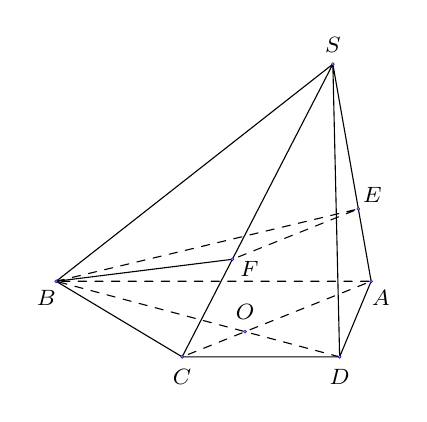
\begin{tikzpicture}[scale=0.8,>=stealth,font=\footnotesize,line join=round,line cap=round,declare function={h=3.5;}]
		 \path
			 (0,0) coordinate (A)
			 (-5,0) coordinate (B)
			 (-3,-1.2) coordinate (C)
			(barycentric  cs:A=1,C=2,B=-1) coordinate (D)
			 (A)+(100:h) coordinate (S)
			(intersection  of A--C and B--D) coordinate (O)
			(barycentric cs:A=2,S=1)  coordinate (E)
			(barycentric  cs:C=2,S=1) coordinate (F);
		\draw[dashed] (D)--(B)--(A)--(C) 
			(B)--(E)--(F); 
		 \draw (C)--(S)--(B)--(C)--(D)--(A)--(S)--(D)
			(B)--(F); 
		\foreach \p/\g  in{A/-60,B/-120,C/-90,D/-90,S/90,O/90,E/45,F/-30}
		\shade[shading=ball](\p) circle  (.03) node[shift={(\g:.25)},scale=1]{$\p$};
	\end{tikzpicture}
	} 
	\shortans{0,86} 
	\loigiai{ 
		\begin{center}
			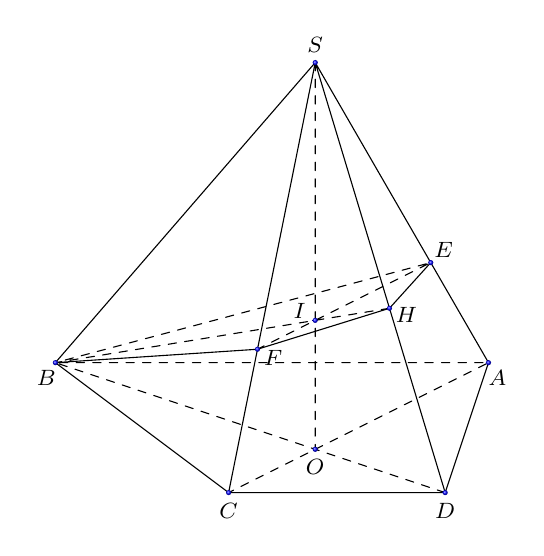
\begin{tikzpicture}[scale=1.1,>=stealth,font=\footnotesize,line join=round,line cap=round,declare function={h=4;}]
					\path 
						(0,0)  coordinate (A)
						(-5,0)  coordinate (B)
						 (-3,-1.5) coordinate (C)
						(barycentric cs:A=1,C=2,B=-1) coordinate (D) 
						(A)+(120:h) coordinate  (S)
						(intersection of A--C and  B--D) coordinate (O)
						(barycentric cs:A=2,S=1)  coordinate (E)
						(barycentric cs:C=2,S=1)  coordinate (F)
						(intersection of E--F and  S--O) coordinate (I)
						 (intersection of B--I and S--D) coordinate (H);
					 \draw[dashed] (D)--(B)--(A)--(C)
						 (H)--(B)--(E)--(F)
						(S)--(O); 
					\draw (C)--(S)--(B)--(C)--(D)--(A)--(S)--(D) 
						(B)--(F)--(H)--(E); 
					\foreach \p/\g  in{A/-60,B/-120,C/-90,D/-90,S/90,O/-90,E/45,F/-30,I/150,H/-20}
					\shade[shading=ball](\p) circle  (.03) node[shift={(\g:.23)},scale=1]{$\p$};
				\end{tikzpicture}
		\end{center}
		Vì $\dfrac{SE}{SA}=\dfrac{SF}{SC}=\dfrac{2}{3}$ nên $EF\parallel AC$. Hơn nữa, $EF\subset(BEF)$, $AC\not\subset(BEF)$ nên $AC$  song song với mặt phẳng $(BEF)$.\\
		Vì $AC$ qua $O$ và song song với  mặt phẳng $(BEF)$ nên $AC\subset(\alpha)$.\\
		Trong $(SAC)$, gọi $I=SO\cap EF$, trong $(SBD)$, gọi  $N=BI\cap SD$. Suy ra $N$ là giao điểm của đường thẳng $SD$ với mặt phẳng $(BEF)$.\\
		Hai mặt phẳng song song $(BEF)$ và $(\alpha)$ bị cắt bởi mặt phẳng thứ ba là $(SCD)$ theo hai giao tuyến song song  với nhau, tức là $Ct\parallel FN$.\\
		Trong $(SCD)$, $Ct$ cắt $SD$  tại $P$. Khi đó, $P$ là giao điểm của $SD$ với $(\alpha)$.\\
		Trong hình thang $ABCD$, do $AB\parallel CD$ và $AB=2CD$ nên  $\dfrac{BO}{OD}=\dfrac{AB}{CD}=2$ $\Rightarrow$ $\dfrac{BO}{BD}=\dfrac{2}{3}$.\\
		Trong tam giác $SAC$, có $EF\parallel AC$ nên  $\dfrac{SE}{SA}=\dfrac{SI}{SO}=\dfrac{2}{3}$ $\Rightarrow$ $\dfrac{IS}{IO}=2$.\\
		Xét tam giác  $SOD$ với cát tuyến $NIB$, ta có $\dfrac{NS}{ND}\cdot \dfrac{BD}{BO}\cdot \dfrac{IO}{IS}=1$ $\Rightarrow$ $\dfrac{NS}{ND}=\dfrac{BO}{BD}\cdot \dfrac{IS}{IO}=\dfrac{2}{3}\cdot 2=\dfrac{4}{3}$.\\
		Suy  ra $\dfrac{SN}{SD}=\dfrac{4}{7}$. \hfill $(1)$\\
		Lại có $\dfrac{SN}{SP}=\dfrac{SF}{SC}=\dfrac{2}{3}$. \hfill  $(2)$\\
		 Từ $(1)$ và $(2)$ suy ra $\dfrac{SP}{SD}=\dfrac{6}{7}$.
	 }
\end{ex}

% nguồn: Ok_TraLoiNgan_Lop11_Lan1
\begin{ex}%[1H4C3-4]%[ma:090ec47a]
	Cho hình chóp $S.ABCD$ có đáy $ABCD$ là hình bình hành tâm $O$. Gọi hai điểm $M, N$ lần lượt trên các cạnh $SB, SC$ sao cho $\dfrac{SN}{SC}=\dfrac{1}{2}$ và $\dfrac{SM}{SB}=\dfrac{2}{3}$. Gọi $P$ là giao điểm của $SD$ và $(AMN)$. Tính tỉ số $\dfrac{SP}{SD}$ (kết quả làm tròn đến hàng phần  trăm).\\
	\shortans{0,67} 
	\loigiai{ 
	 \immini{Trong mặt phẳng $(SAC)$, gọi $K=SO\cap AN$.\\
		Trong mặt phẳng $(SBD)$, gọi $P=SD\cap MK$.  \\
		Mà $MK\subset (AMN)$ nên $P=SD\cap  (AMN)$. \\
		Tam giác $SAC$ có $AN$ và $SO$ là  hai đường trung tuyến nên $K$ là trọng tâm của tam giác $SAC$. Suy ra $\dfrac{SK}{SO}=\dfrac{2}{3}$. $\quad \quad (1)$\\
		Mà $\dfrac{SM}{SB}=\dfrac{2}{3}$. $ \quad \quad (2)$ \\ 
		Từ $(1)$ và $(2)$,  suy ra $ \dfrac{SK}{SO}=\dfrac{SM}{SB}$.\\
		 }{
		\begin{tikzpicture}[scale=1,>=stealth,font=\footnotesize,line join=round,line cap=round]
				\coordinate (B)  at (0,0);
				 \coordinate (A) at (-1.6,-1);
				\coordinate  (C) at (3.5,0);
				\coordinate (D)  at ($(C)-(B)+(A)$);
				\coordinate (S) at  ($(A)+(1.2,4.5)$);
				 \coordinate (M) at ($(S)!0.67!(B)$);
				 \coordinate (N) at ($(S)!0.5!(C)$);
				\draw  (S)--(A)--(D)--(C)--(S)--(D);
				\draw[dashed]  (A)--(B)--(C)
					(S)--(B) 
					(A)--(C) 
					(B)--(D) 
					 (A)--(M)--(N)--cycle;
				\coordinate (O) at (intersection of  A--C and B--D);
				\coordinate (K) at (intersection of S--O and  A--N);
				\coordinate (P) at (intersection of M--K and  S--D);
				 \draw[dashed] (S)--(O)
					 (M)--(P);
				\foreach \p/\r  in {S/90,A/170,B/-90,C/-45,D/-30,M/135,N/100,O/-90,K/70,P/40}
				 \fill (\p) circle (1pt) node[shift={(\r:3mm)}]{$\p$};
			\end{tikzpicture}
		 }
		\noindent 
		Theo định lí Ta-lét đảo trong tam giác $SBO$,  ta có
		$KM \parallel  BO$.\\
		Do đó $\dfrac{SP}{SD}=\dfrac{SK}{SO}=\dfrac{2}{3}\approx 0{,}67$. 
	 }
\end{ex}


%%%%%%%%%%%%%%%% TỰ LUẬN %%%%%%%%%%%%%%%%

% nguồn: Ok_TuanLuan_Toan11_Lan2
\begin{ex}%[1H4H3-4]%[ma:8d10be19]
	Cho tứ diện $ABCD$ có $G$ là trọng tâm tam giác $BCD$. Biết mặt phẳng $(\alpha)$ chứa $BG$ và song song với  đường thẳng $AC$. Tìm giao điểm $K$ của $AD$ và mặt phẳng $(\alpha)$.
	 \loigiai{
		\begin{center}
			\begin{tikzpicture}[line join = round,line cap = round,>=stealth,font=\footnotesize,scale=1,declare function={ab=3; bc=2.2; bd=4.5; gocB=-60; gn=70;}]
					 \path
						 (0,0) coordinate (B)
						 (gn:ab) coordinate (A)
						 (bd,0) coordinate (D)
						(gocB:bc) coordinate (C) 
						($(D)!0.5!(C)$)  coordinate (I)
						($(B)!2/3!(I)$) coordinate (G) 
						 ($(A)!0.5!(D)$) coordinate (K);
					\draw (A)--(B)--(C)--(D)--(A)--(C) 
						 (K)--(I);
					\draw[dashed]  (D)--(B)
						 (K)--(B)--(I);
					\foreach \x/\gm in  {A/90,B/180,C/-90,D/0,I/-70,K/40,G/-90} \fill (\x) circle (1pt)
						 ($(\x)+(\gm:3.5mm)$) node{$\x$};
				\end{tikzpicture}
		\end{center}
		 Gọi $I$ là trung điểm của $CD$.\\
		Ta có $\heva{& I\in(\alpha) \cap(ACD) \\  & AC\parallel(\alpha) \\ & AC\subset(ACD)} \Rightarrow(\alpha) \cap(ACD)=Ix \parallel AC$.\\
		Trong mặt phẳng $(ACD)$  gọi $Ix \cap AD=K$.\\
		 Ta có $\heva{& K\in AD \\ & K\in Ix \subset(\alpha) \Rightarrow K\in(\alpha)} \Rightarrow K=AD\cap(\alpha)$.
	} 
\end{ex}

% nguồn: Ok_TuanLuan_Toan11_Lan2
\begin{ex}%[1H4V3-4]%[ma:2e68012c]
	Cho hình chóp $S\cdot ABCD$ có đáy $ABCD$ là hình thang có đáy lớn là $AB$. Gọi $M$ là một điểm trên $CD$ và $(\alpha)$ là mặt phẳng qua $M$ và song song với $SA$ và  $BC$. Tìm giao điểm $Q$ của $SC$ và $(\alpha)$.
	 \loigiai{
		\begin{center}
			\begin{tikzpicture}[line join = round,line cap = round,>=stealth,font=\footnotesize,scale=1,declare function={ad=2; ab=4; cd=2.1; gocA=-40; sa=3.5;}]
					 \path
						(0,0) coordinate (A) 
						(ab,0) coordinate (B) 
						 (gocA:ad) coordinate (D)
						 ($(D)+(cd,0)$) coordinate (C)
						(50:sa)  coordinate (S)
						(intersection of A--C  and B--D) coordinate (O)
						($(C)!0.7!(D)$) coordinate  (M)
						($(M)-(C)+(B)$) coordinate  (N)
						(intersection of A--C and M--N) coordinate  (I)
						 ($(S)-(A)+(I)$) coordinate (Q1)
						(intersection of I--Q1 and S--C)  coordinate (Q);
					\draw  (S)--(A)--(D)--(C)--(B)--(S)--(D)
						(S)--(C); 
					\draw[dashed]  (A)--(B)
						(A)--(C) 
						 (M)--(N)
						(I)--(Q); 
					 \foreach \x/\gm in {A/180,B/0,C/-90,D/-90,S/90,N/90,M/-90,Q/20,I/200} \draw[fill] (\x) circle (1pt)
						 ($(\x)+(\gm:3.5mm)$) node{$\x$};
				\end{tikzpicture}
		\end{center}
		Ta có $\heva{& (\alpha) \parallel BC,  BC\subset(ABCD) \\ & M\in(\alpha) \cap(ABCD)} \Rightarrow(\alpha) \cap(ABCD)=MN\parallel BC$ và $N\in AB$.\\
		Gọi $I$ là giao điểm của $AC$ và  $MN$ ta có $\heva{&SA\parallel(\alpha) \\ & SA\subset(SAC) \\ & I\in(\alpha) \cap(SAC)} \Rightarrow(\alpha) \cap(SAC)=Ix \parallel SA$.\\
		Trong mặt phẳng ($SAC$) gọi $Q$ là giao điểm của  $Ix$ và $SC$.\\
		Ta có $\heva{&Q\in SC\\&Q\in  Ix \subset(\alpha) \Rightarrow I\in(\alpha)} \Rightarrow Q=SC\cap(\alpha)$.
	} 
\end{ex}

% nguồn: Ok_TuanLuan_Toan11_Lan2
\begin{ex}%[1H4V3-4]%[ma:6d8d238a]
	Cho hình chóp $S.ABCD$ có đáy $ABCD$ là hình thang đáy lớn $AB$. Gọi $M$ là một điểm trên $CD$ và  ($\alpha$) là mặt phẳng qua $M$ và song song với $SA$ và $BC$. Tìm giao điểm $Q$ của $SC$ và mặt phẳng $(\alpha)$.
	\loigiai{ 
		\begin{center}
			\begin{tikzpicture}[scale=1,font=\footnotesize,line join=round,line cap=round,>=stealth]
					\path 
						 (0,0) coordinate (A)
						(5,0) coordinate (B) 
						(2,-1) coordinate (D) 
						 (4,-1) coordinate (C)
						(1,3.5) coordinate (S) 
						($(B)+(-1.5,0)$) coordinate (N) 
						($(C)+(-1.5,0)$)  coordinate (M)
						(intersection  of A--C and M--N) coordinate (I)
						 ($(S)+(I)-(A)$) coordinate (K)
						(intersection of I--K and S--C) coordinate (Q); 
					\draw  (S)--(A)--(D)--(C)--(B)--(S)--(C)
						 (S)--(D);
					\draw [dashed]  (C)--(A)--(B)
						(M)--(N) 
						 (I)--(Q);
					\foreach  \d/\g in {A/135,D/-135,C/-45,B/45,S/90,M/-90,N/45,I/135,Q/180}
					\fill (\d) circle (1pt) + (\g:.3) node{$\d$}; 
				\end{tikzpicture}
		\end{center}
		Ta có $\heva{&(\alpha)\parallel BC,BC\subset(ABCD)\\&M\in(\alpha)\cap(ABCD)}\Rightarrow(\alpha)\cap(ABCD)=MN\parallel BC$ và $(N\in AB)$.\\ 
		Gọi $I$  là giao điểm của $AC$ và $MN$ ta có $\heva{&SA\parallel (\alpha)\\&SA\subset(SAC)\\&I\in(\alpha)\cap(SAC)}\Rightarrow(\alpha)\cap(SAC)=Ix\parallel SA$.\\
		Trong mặt phẳng  ($SAC$) gọi $Q$ là giao điểm của $Ix$ và $SC$.\\
		Ta có $\heva{&Q\in SC\\&Q\in Ix\subset(\alpha)\Rightarrow I\in(\alpha)}\Rightarrow  Q=SC\cap(\alpha)$.
	} 
\end{ex}
